\documentclass{article}\usepackage[]{graphicx}\usepackage[]{color}
%% maxwidth is the original width if it is less than linewidth
%% otherwise use linewidth (to make sure the graphics do not exceed the margin)
\makeatletter
\def\maxwidth{ %
  \ifdim\Gin@nat@width>\linewidth
    \linewidth
  \else
    \Gin@nat@width
  \fi
}
\makeatother

\definecolor{fgcolor}{rgb}{0.345, 0.345, 0.345}
\newcommand{\hlnum}[1]{\textcolor[rgb]{0.686,0.059,0.569}{#1}}%
\newcommand{\hlstr}[1]{\textcolor[rgb]{0.192,0.494,0.8}{#1}}%
\newcommand{\hlcom}[1]{\textcolor[rgb]{0.678,0.584,0.686}{\textit{#1}}}%
\newcommand{\hlopt}[1]{\textcolor[rgb]{0,0,0}{#1}}%
\newcommand{\hlstd}[1]{\textcolor[rgb]{0.345,0.345,0.345}{#1}}%
\newcommand{\hlkwa}[1]{\textcolor[rgb]{0.161,0.373,0.58}{\textbf{#1}}}%
\newcommand{\hlkwb}[1]{\textcolor[rgb]{0.69,0.353,0.396}{#1}}%
\newcommand{\hlkwc}[1]{\textcolor[rgb]{0.333,0.667,0.333}{#1}}%
\newcommand{\hlkwd}[1]{\textcolor[rgb]{0.737,0.353,0.396}{\textbf{#1}}}%
\let\hlipl\hlkwb

\usepackage{framed}
\makeatletter
\newenvironment{kframe}{%
 \def\at@end@of@kframe{}%
 \ifinner\ifhmode%
  \def\at@end@of@kframe{\end{minipage}}%
  \begin{minipage}{\columnwidth}%
 \fi\fi%
 \def\FrameCommand##1{\hskip\@totalleftmargin \hskip-\fboxsep
 \colorbox{shadecolor}{##1}\hskip-\fboxsep
     % There is no \\@totalrightmargin, so:
     \hskip-\linewidth \hskip-\@totalleftmargin \hskip\columnwidth}%
 \MakeFramed {\advance\hsize-\width
   \@totalleftmargin\z@ \linewidth\hsize
   \@setminipage}}%
 {\par\unskip\endMakeFramed%
 \at@end@of@kframe}
\makeatother

\definecolor{shadecolor}{rgb}{.97, .97, .97}
\definecolor{messagecolor}{rgb}{0, 0, 0}
\definecolor{warningcolor}{rgb}{1, 0, 1}
\definecolor{errorcolor}{rgb}{1, 0, 0}
\newenvironment{knitrout}{}{} % an empty environment to be redefined in TeX

\usepackage{alltt}
\usepackage[utf8]{inputenc}
\usepackage{hyperref}
\hypersetup{
    linktocpage,
    colorlinks=true, 
    linkcolor=blue,
    citecolor=blue,
    filecolor=blue,
    urlcolor=blue
}
\IfFileExists{upquote.sty}{\usepackage{upquote}}{}
\begin{document}


\title{Transcription vs Metilation}
\author{Lucas Michel Todó}
\maketitle
\tableofcontents
\clearpage


\section{Generalitats}
En tots els gràfics la columna de més a l'esquerra correspon als valors de diferència de transcripció (1.2B - 10G). Les columnes següents corresponen a algun paràmetre relacionat amb la metilació (percentatge del gen metilat, coverage mitjà...). En alguns casos hi ha valor de metilació per a 1.2B i per a 10G i en altres una sola columna que correspon a la diferència de metilació.
\section{Heatmaps Percentatge de Coverge}
\subsection{Gene-body}
\begin{knitrout}
\definecolor{shadecolor}{rgb}{0.969, 0.969, 0.969}\color{fgcolor}

{\centering 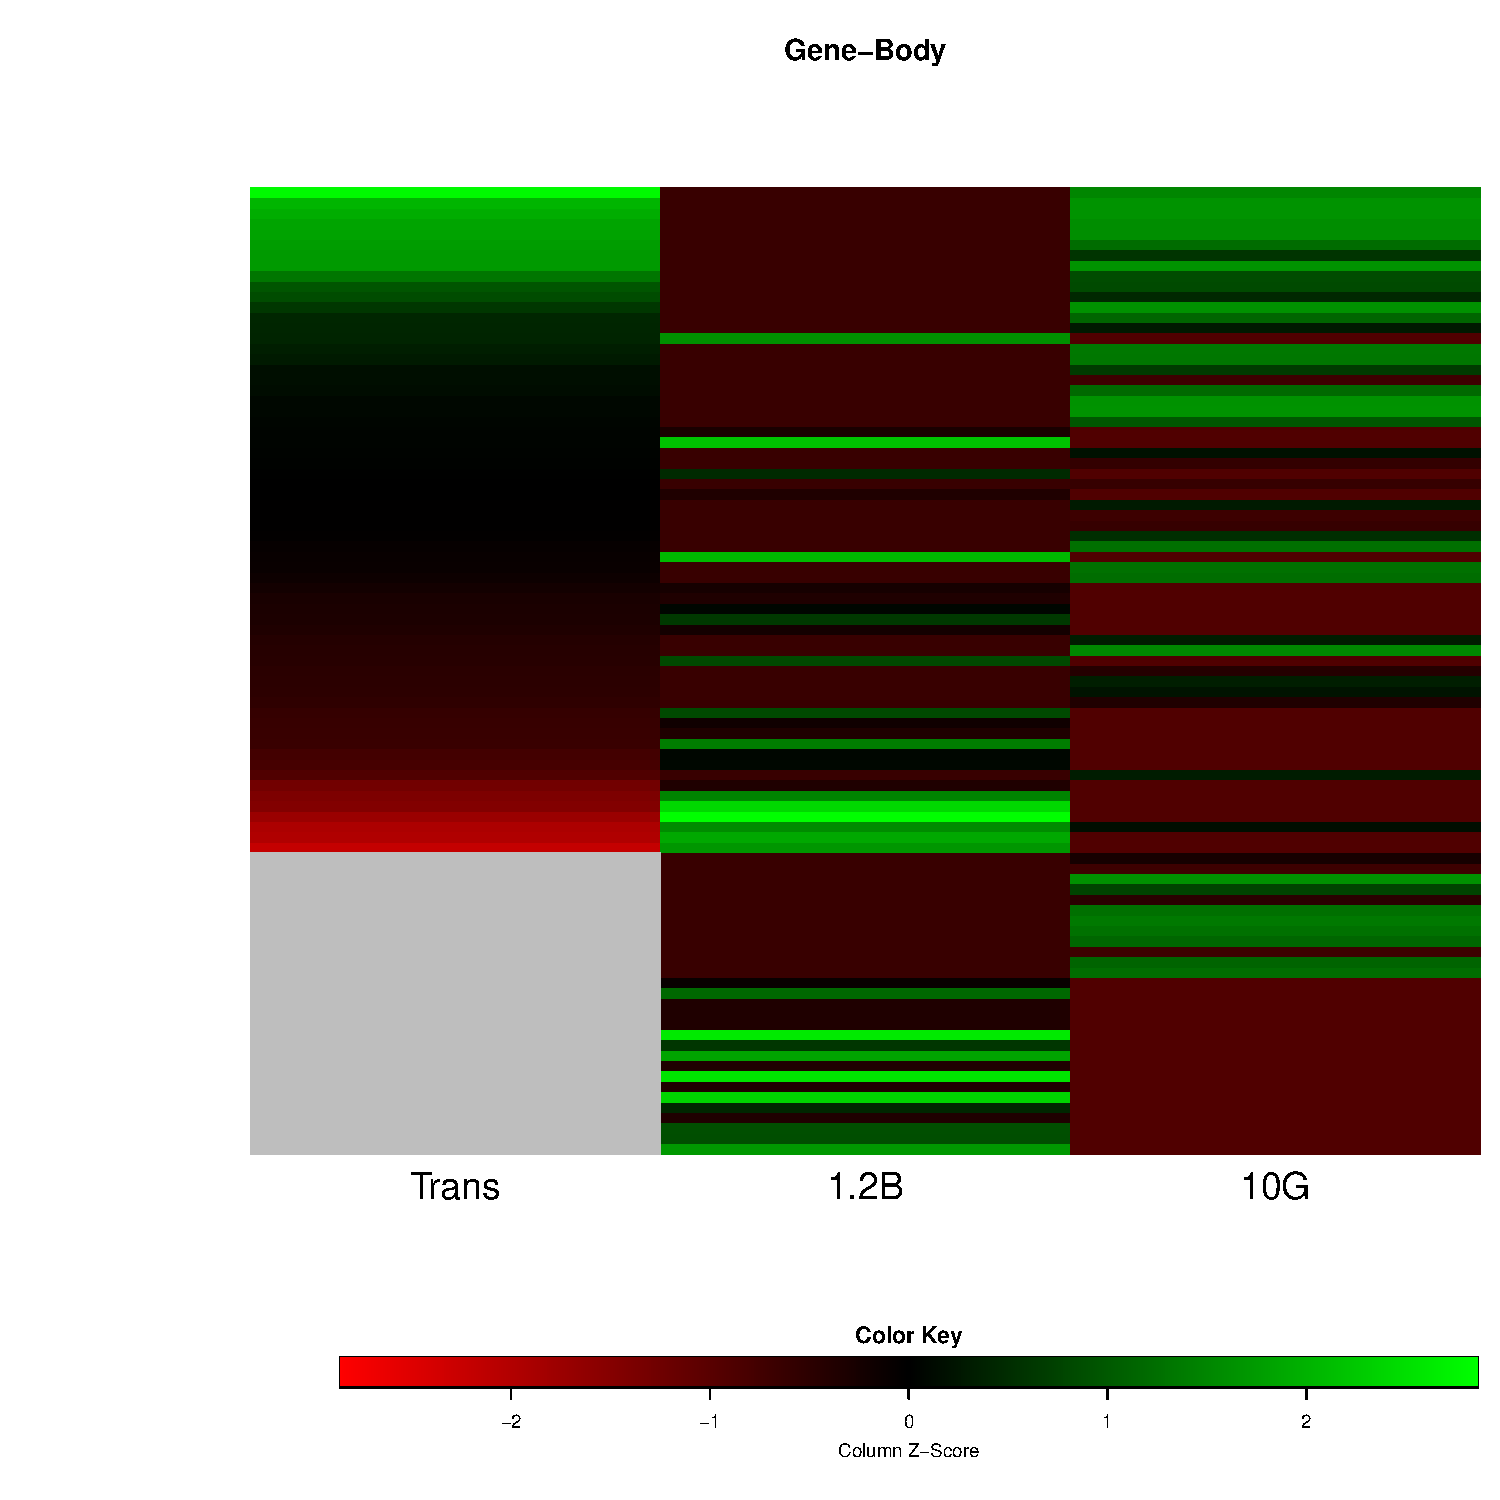
\includegraphics[width=.9\linewidth]{figure/minimal-heatmap_gene-1} 

}



\end{knitrout}
\clearpage
\subsection{TSS}
\begin{knitrout}
\definecolor{shadecolor}{rgb}{0.969, 0.969, 0.969}\color{fgcolor}

{\centering 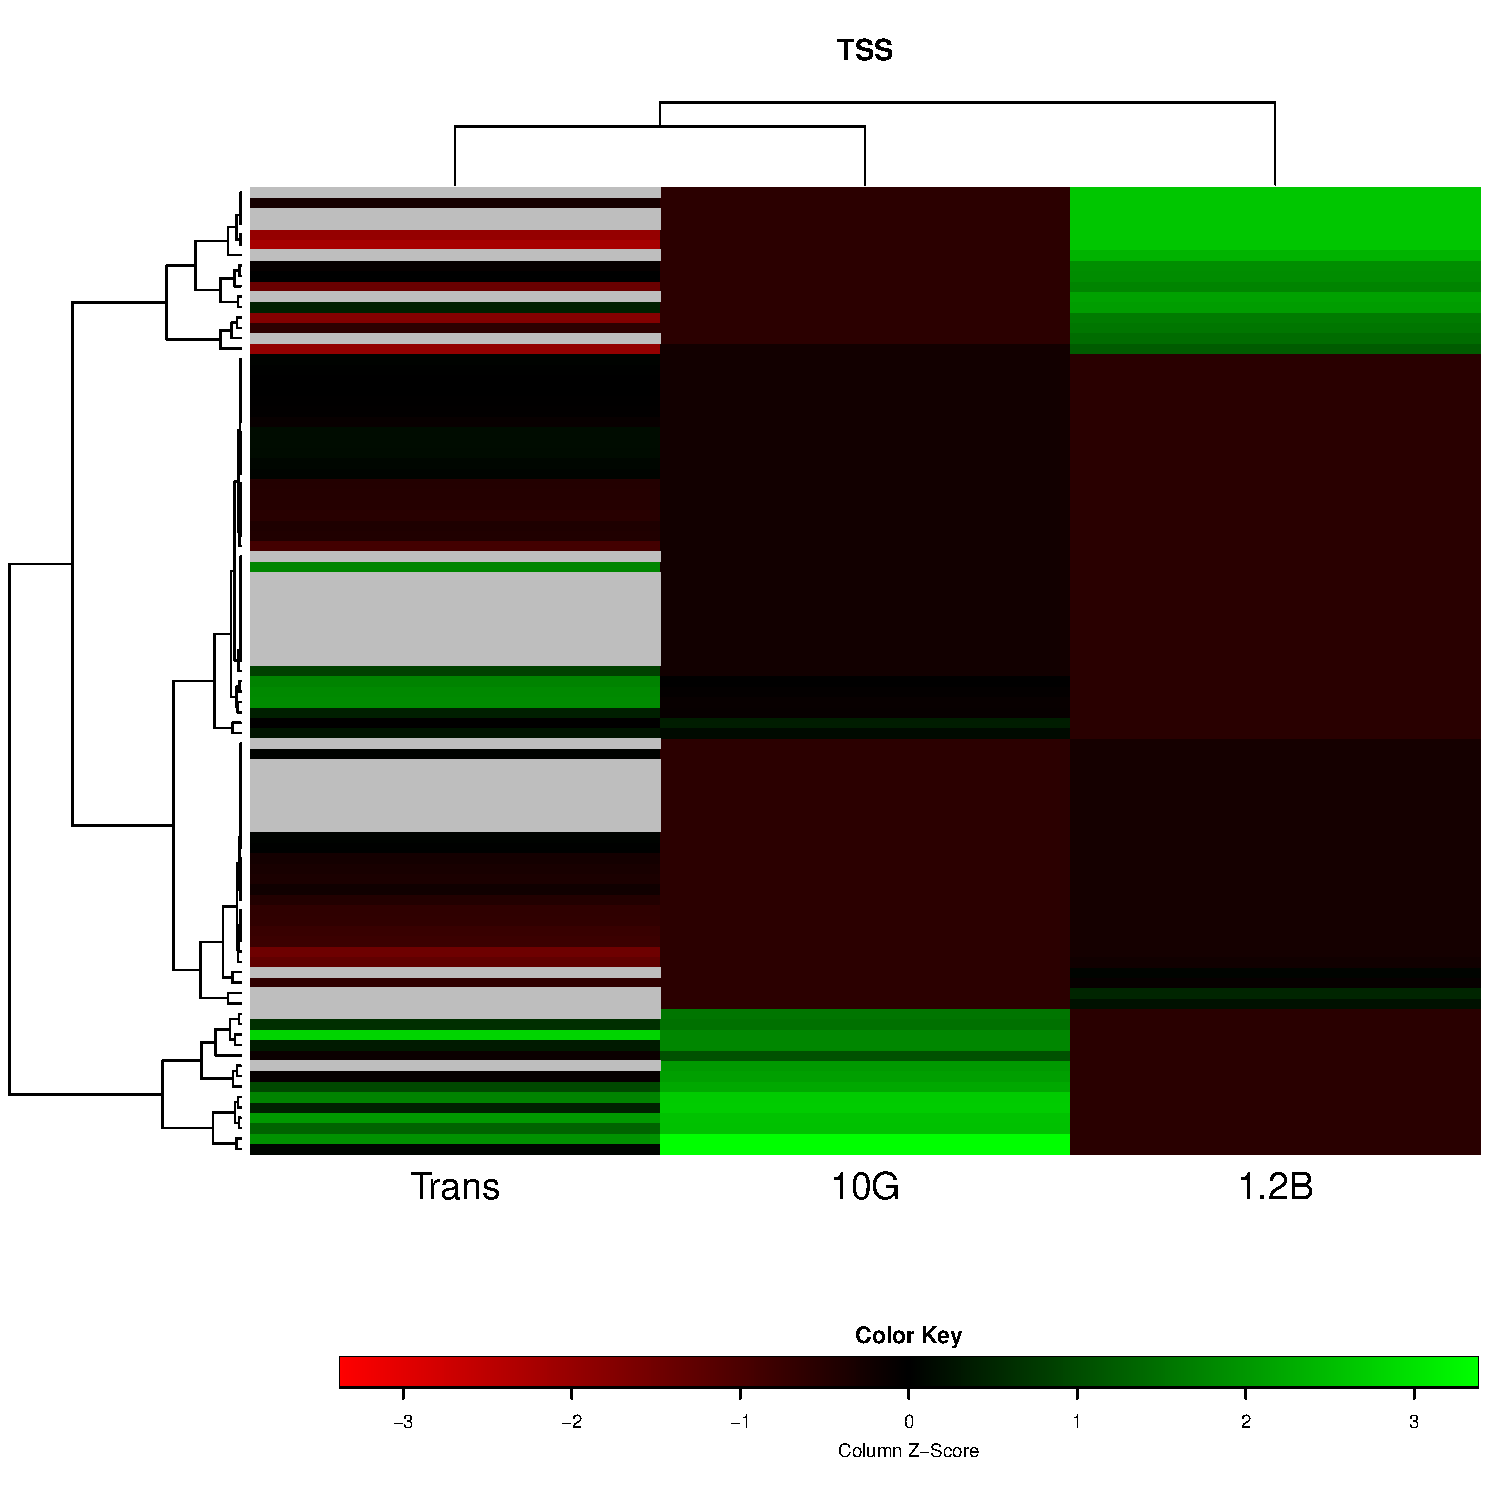
\includegraphics[width=.9\linewidth]{figure/minimal-heatmap_tss-1} 

}



\end{knitrout}
\clearpage
\subsection{Gene + TSS}
\begin{knitrout}
\definecolor{shadecolor}{rgb}{0.969, 0.969, 0.969}\color{fgcolor}

{\centering 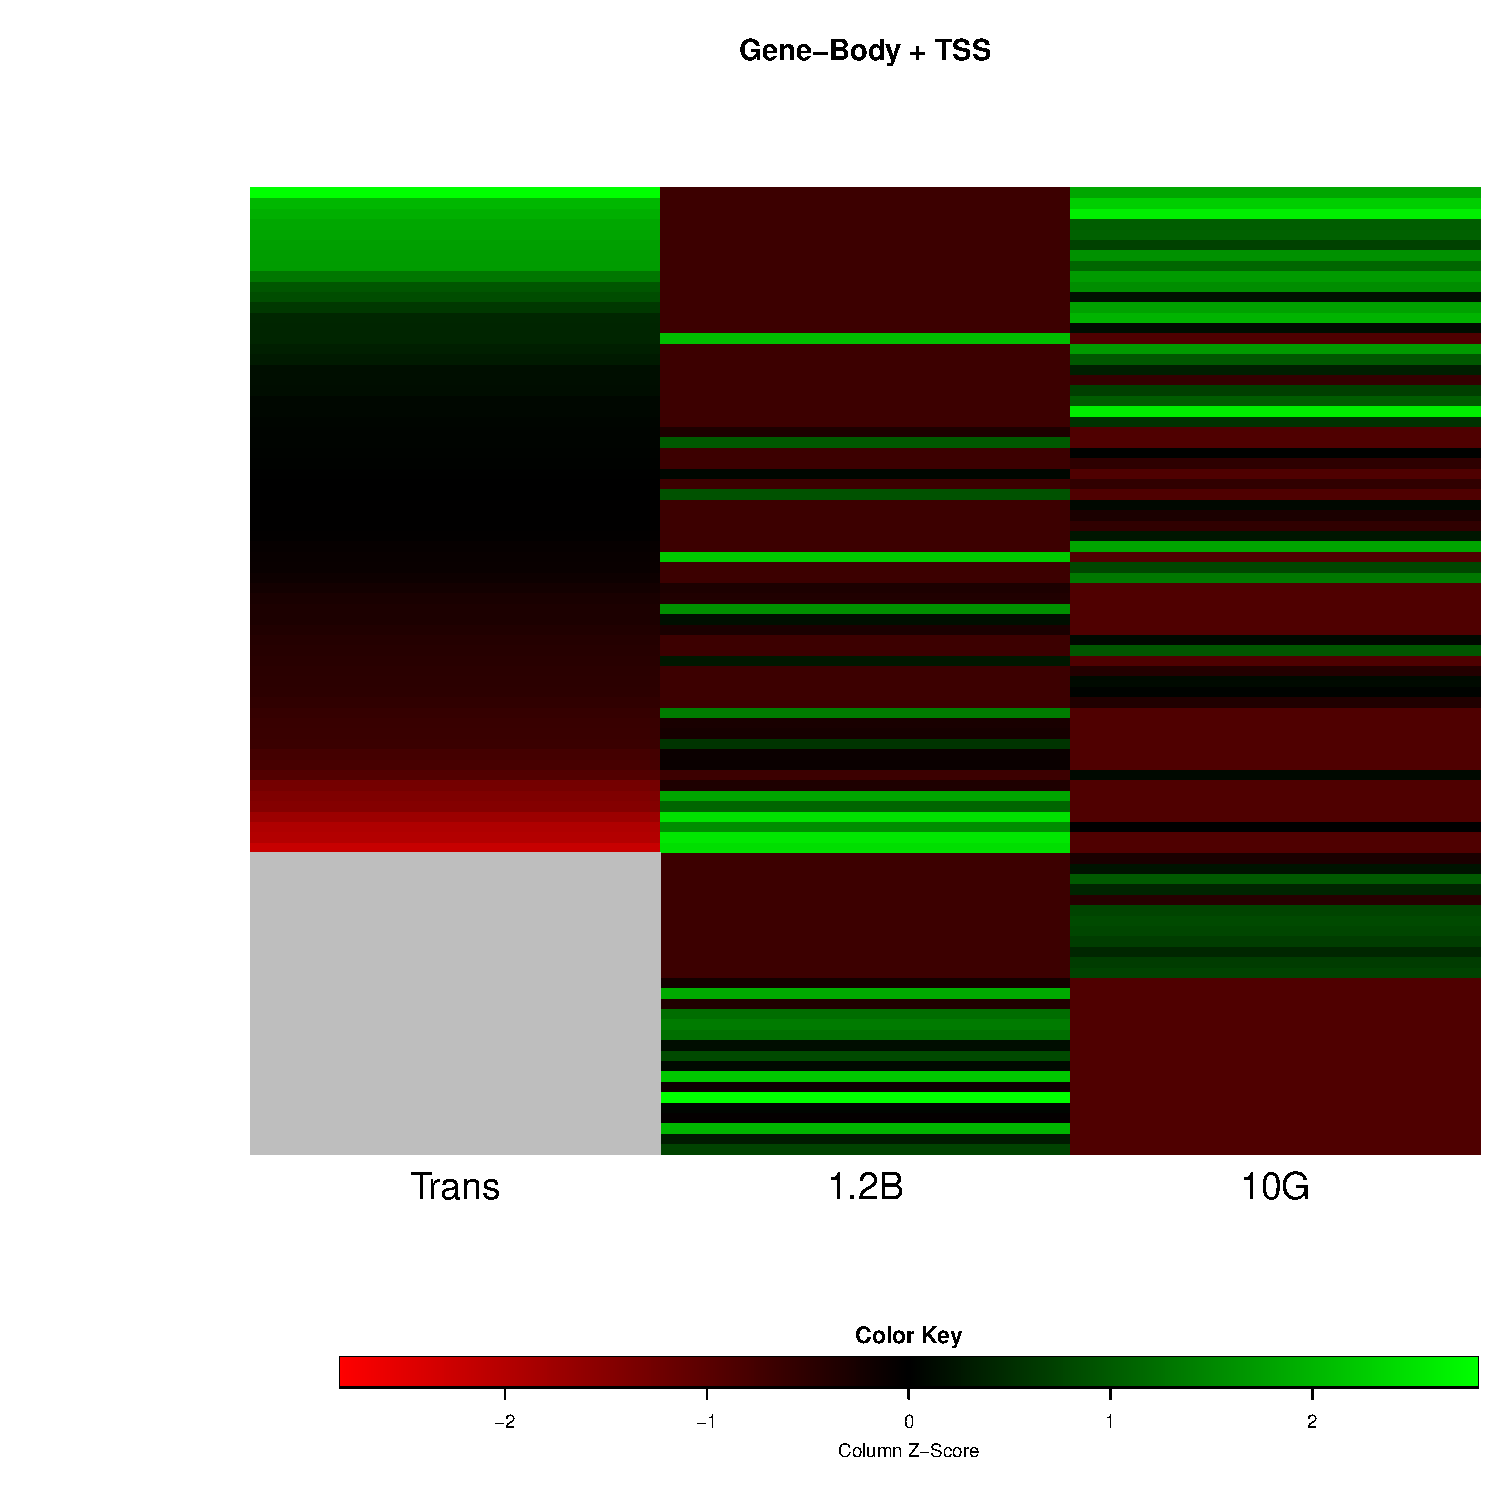
\includegraphics[width=.9\linewidth]{figure/minimal-heatmap_gene_tss-1} 

}



\end{knitrout}
\clearpage
\subsection{TTS}
\begin{knitrout}
\definecolor{shadecolor}{rgb}{0.969, 0.969, 0.969}\color{fgcolor}

{\centering 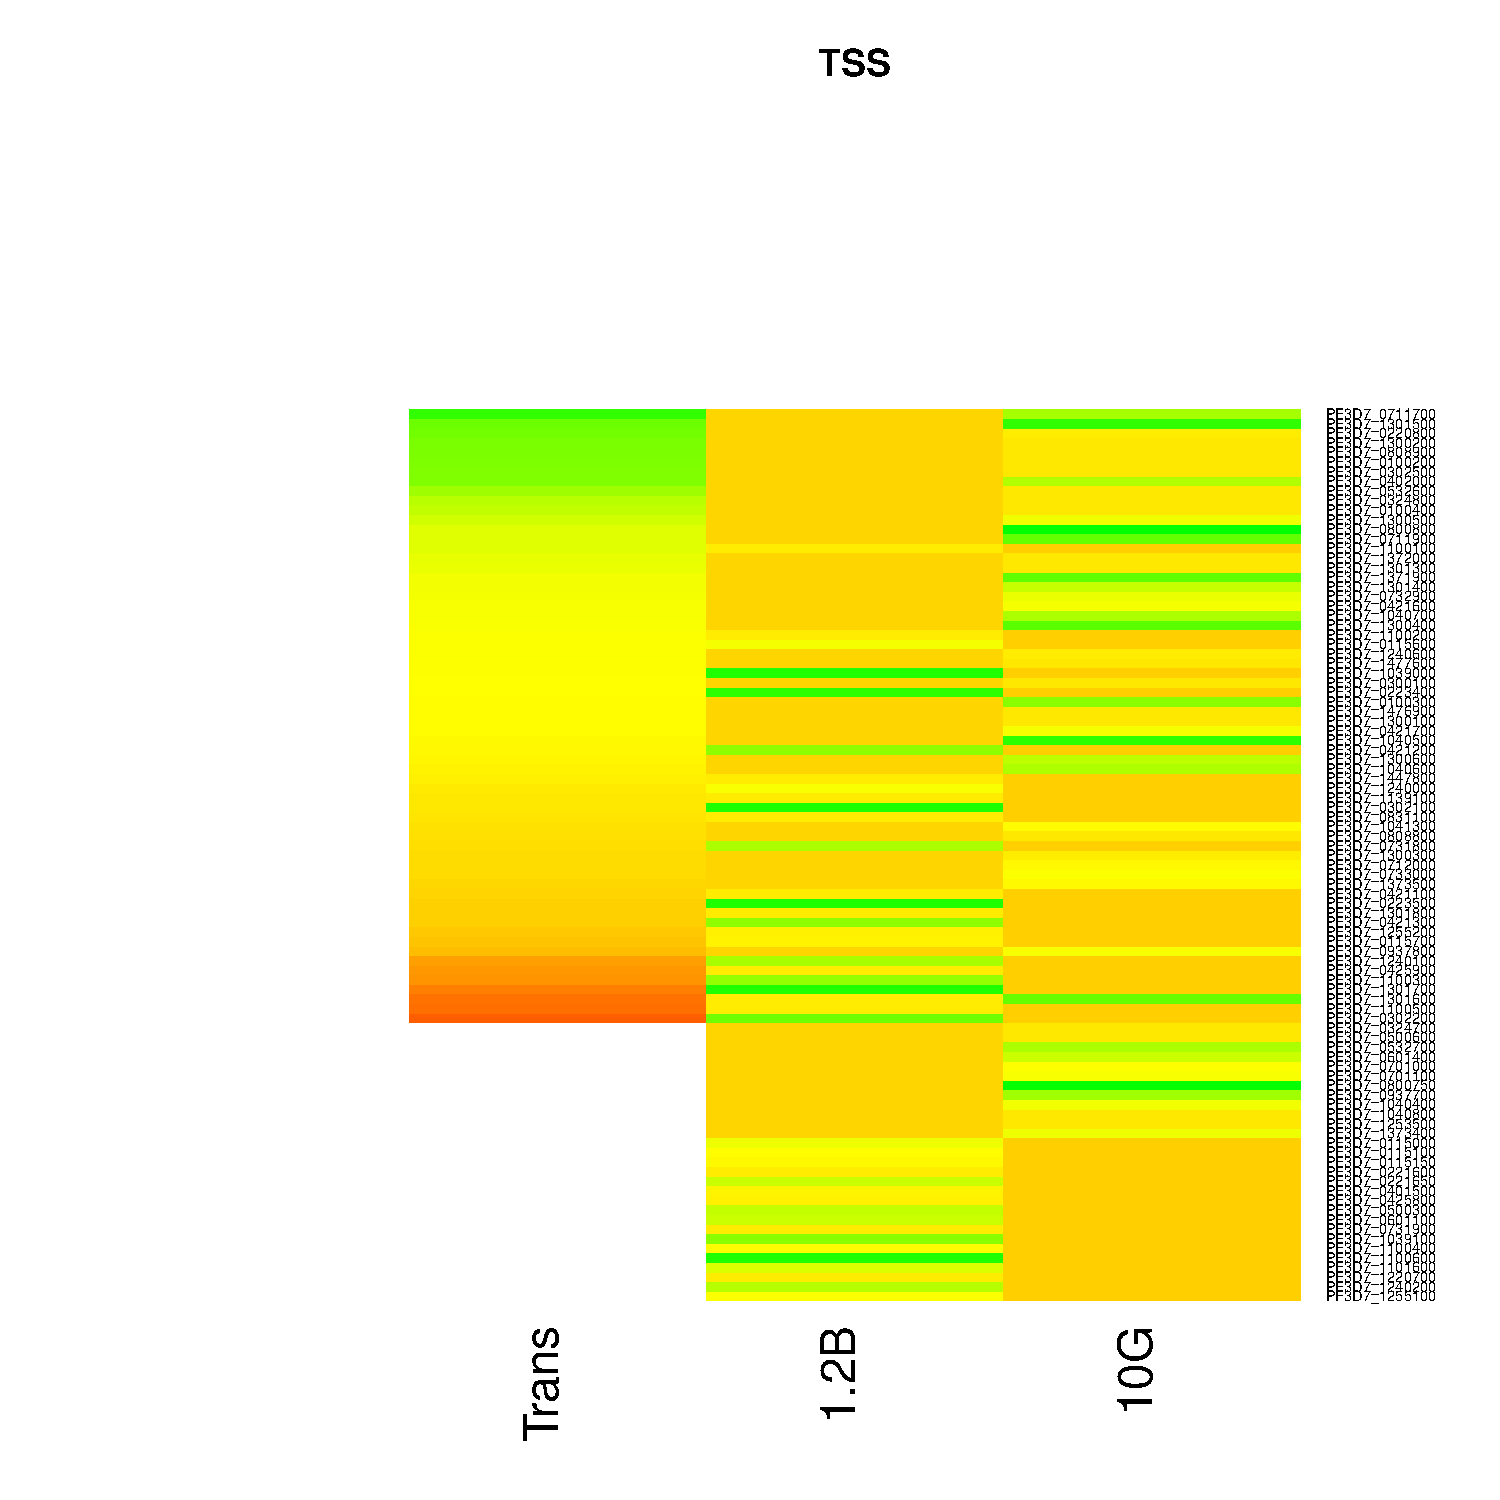
\includegraphics[width=.9\linewidth]{figure/minimal-heatmap_tts-1} 

}



\end{knitrout}
\clearpage
\subsection{TSS+Gene+TTS}
\begin{knitrout}
\definecolor{shadecolor}{rgb}{0.969, 0.969, 0.969}\color{fgcolor}

{\centering 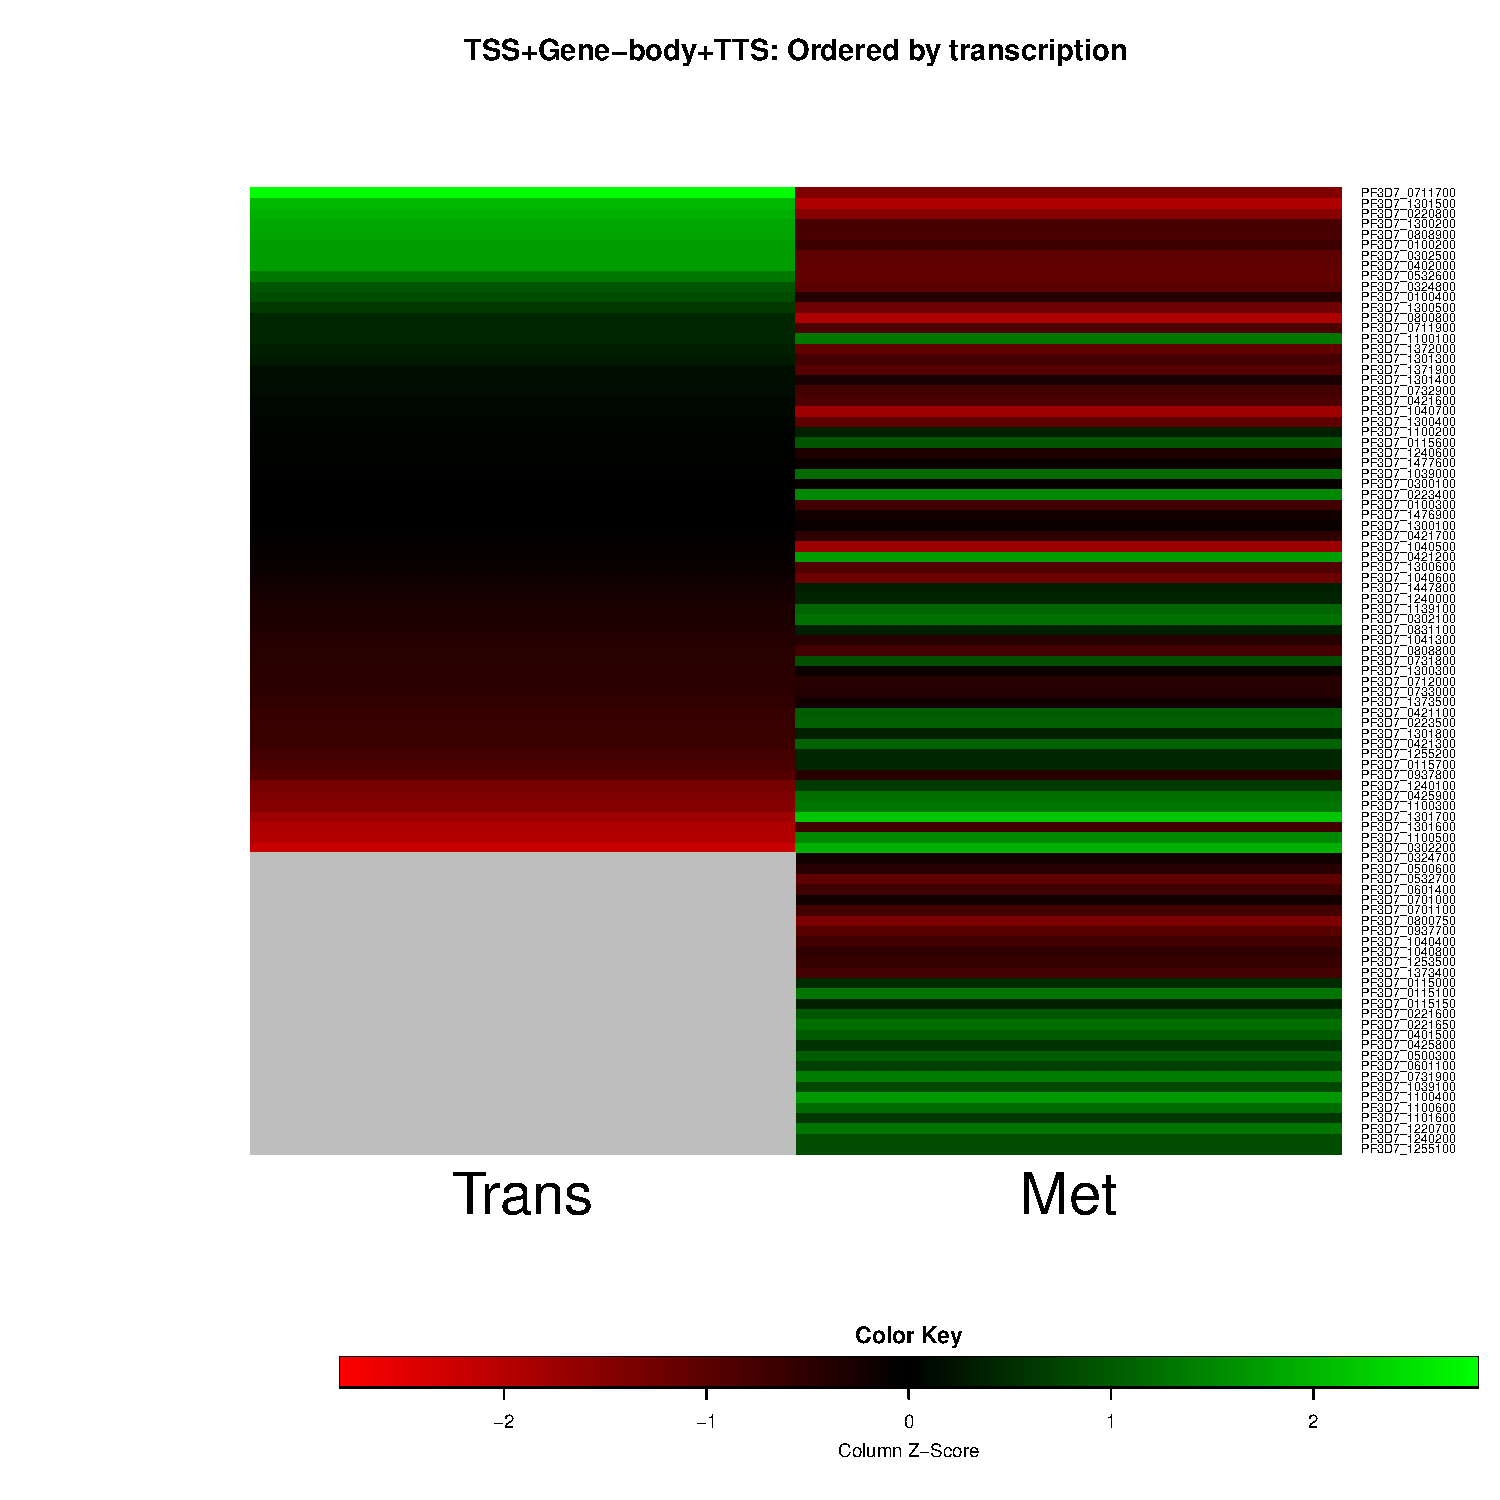
\includegraphics[width=.9\linewidth]{figure/minimal-heatmap_all-1} 

}



\end{knitrout}

\clearpage
\section{Heatmaps Coverge}

\subsection{Coverage Gene Body}
\begin{knitrout}
\definecolor{shadecolor}{rgb}{0.969, 0.969, 0.969}\color{fgcolor}

{\centering 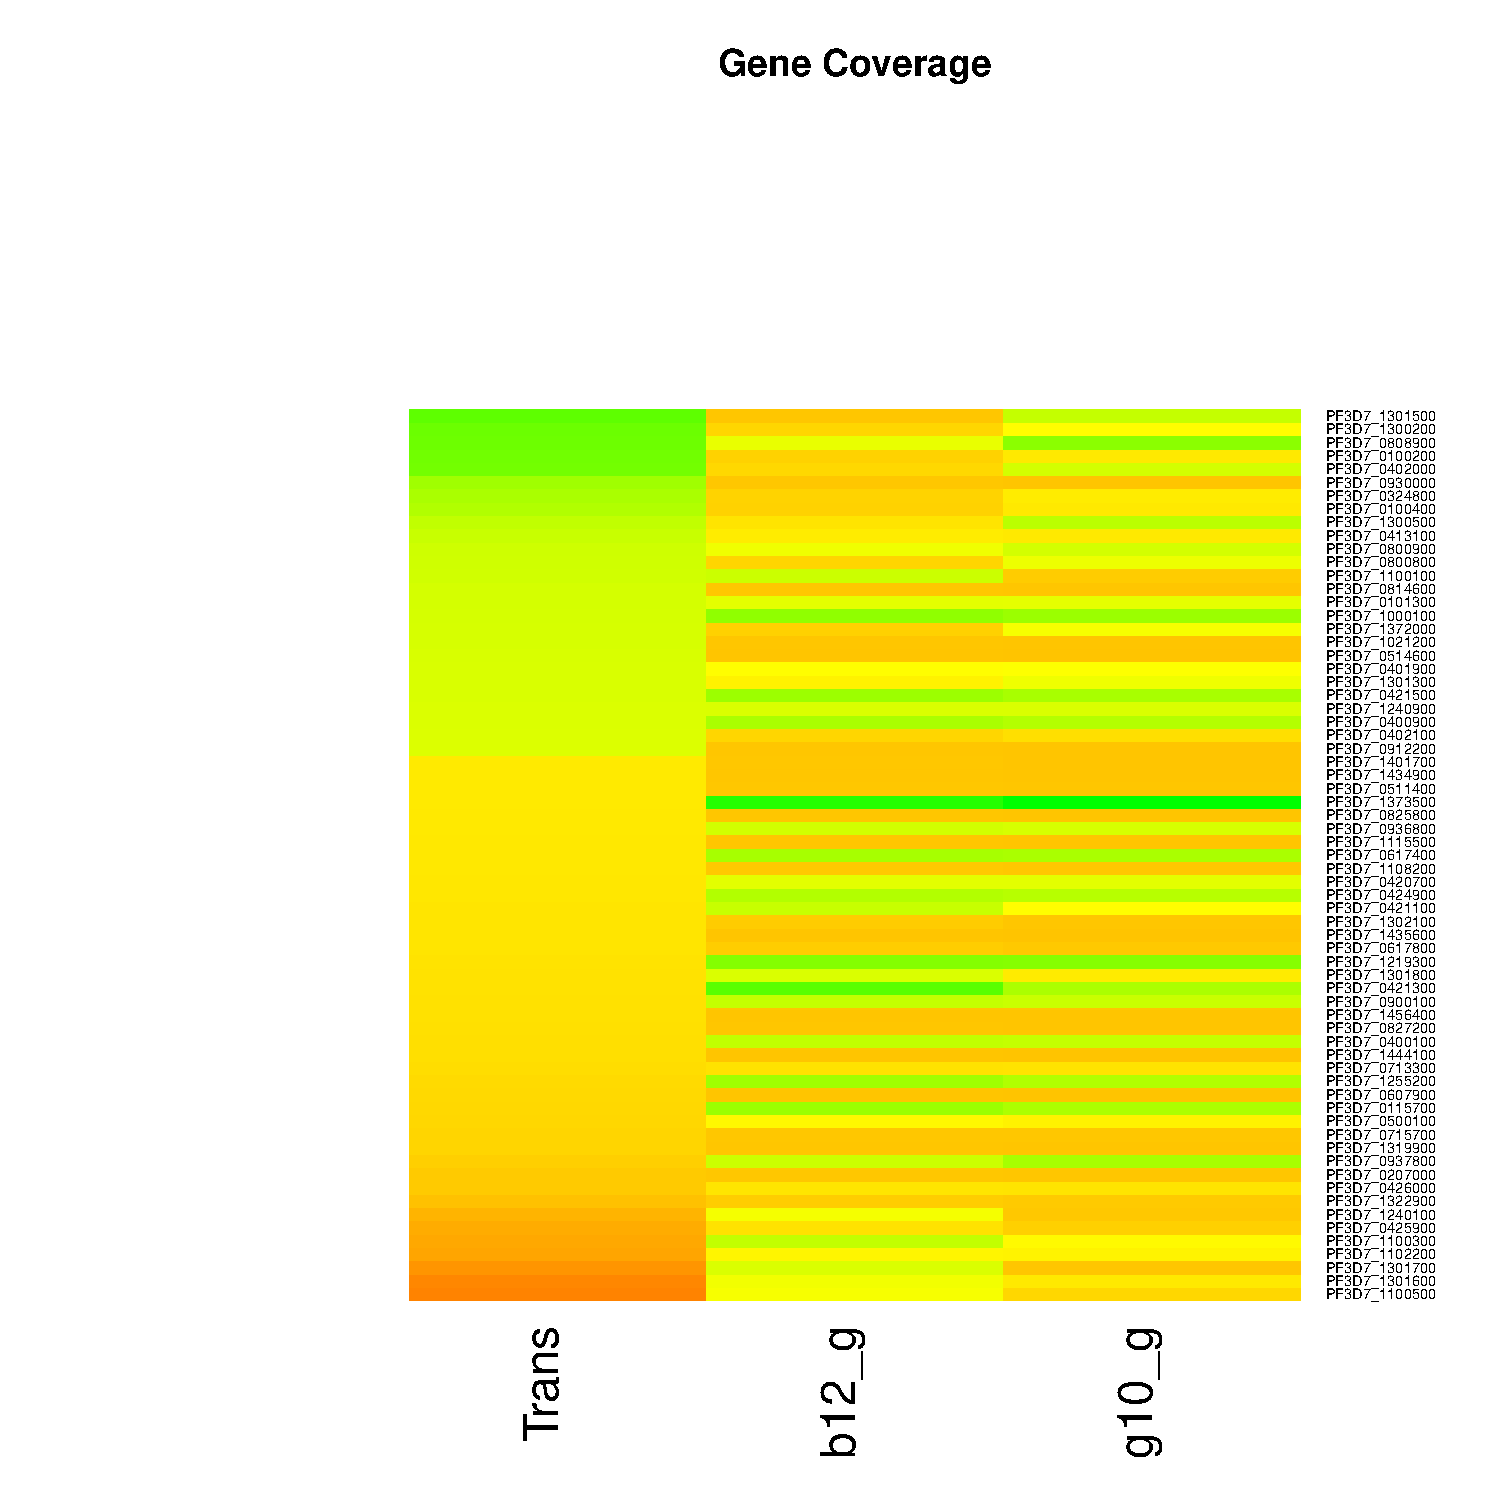
\includegraphics[width=.9\linewidth]{figure/minimal-heat_cov_gene-1} 

}



\end{knitrout}
\clearpage
\subsection{Coverage 5'}
\begin{knitrout}
\definecolor{shadecolor}{rgb}{0.969, 0.969, 0.969}\color{fgcolor}

{\centering 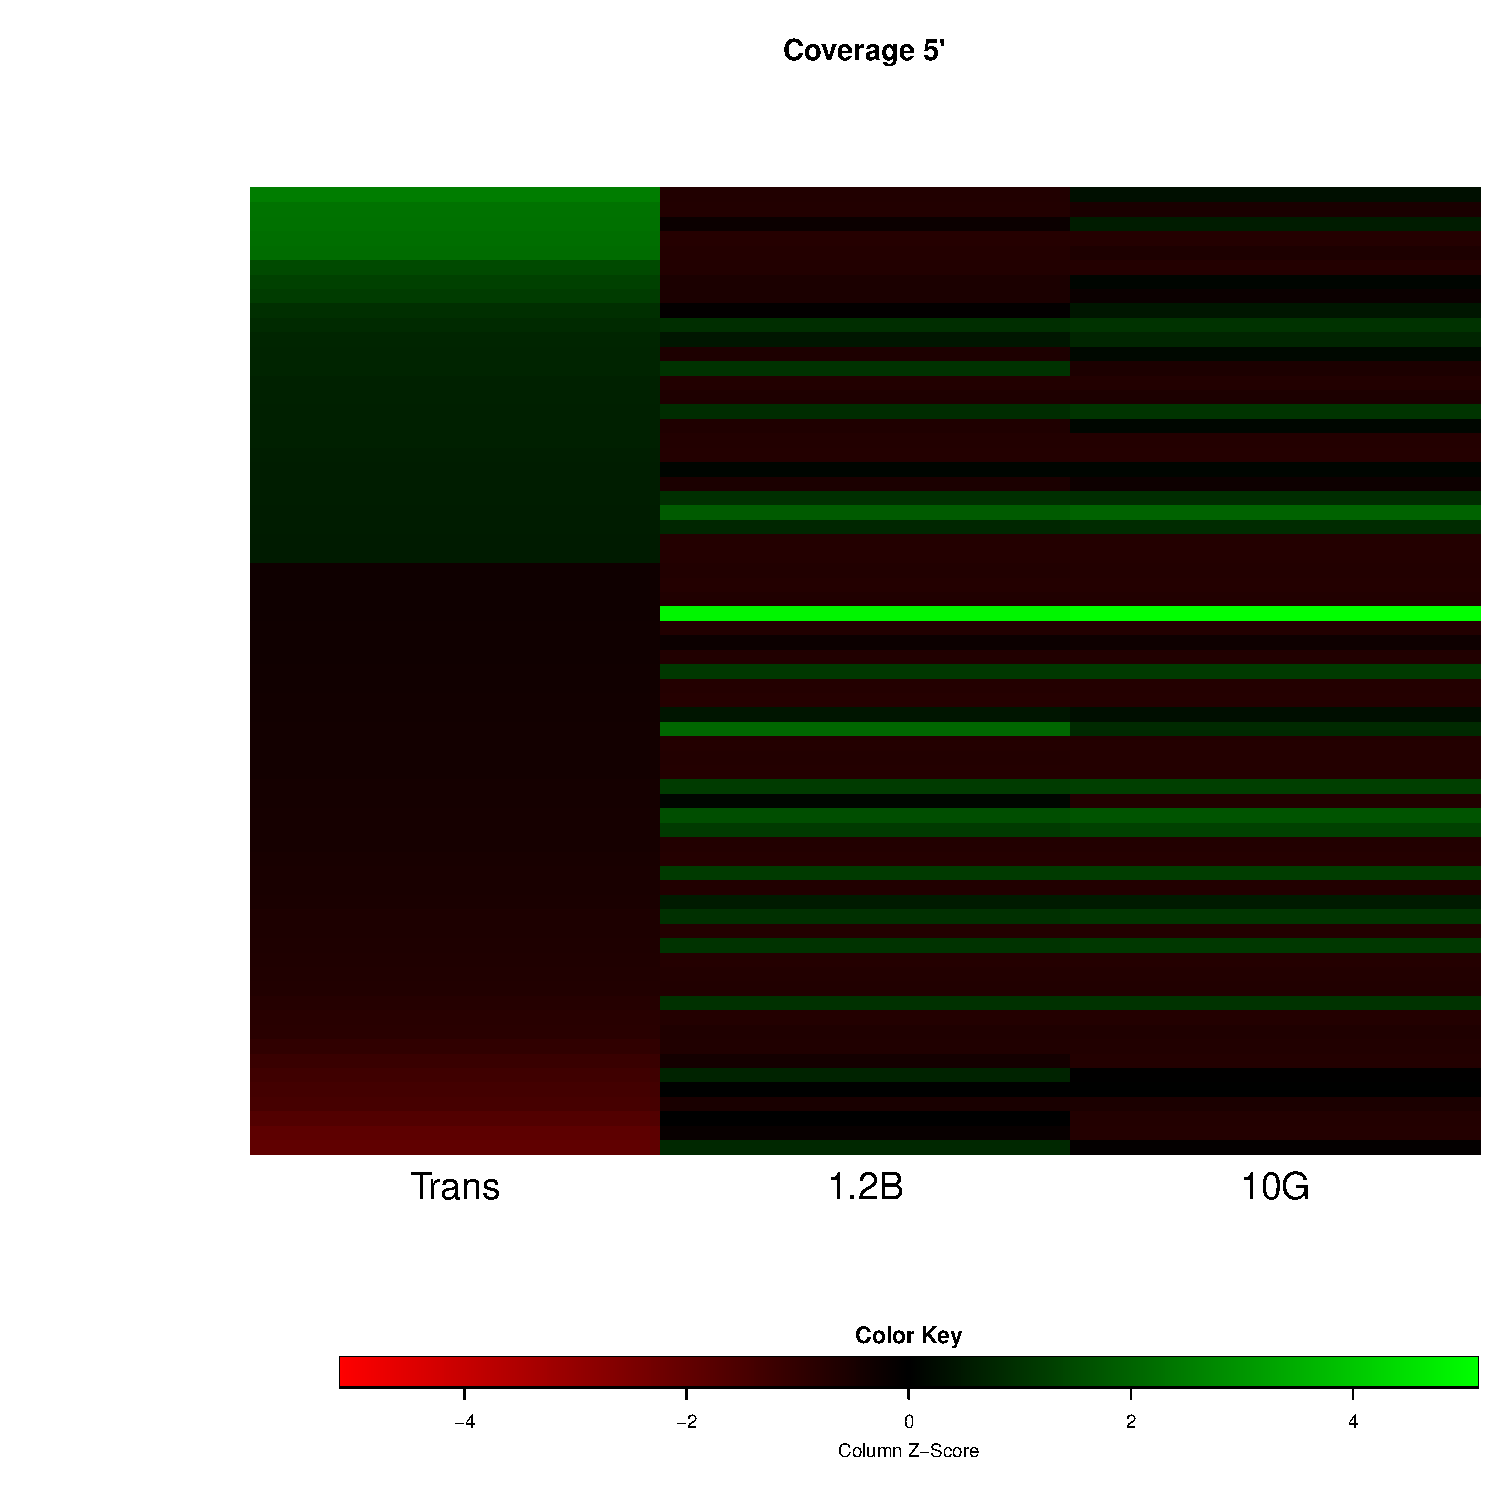
\includegraphics[width=.9\linewidth]{figure/minimal-heat_cov_tss-1} 

}



\end{knitrout}
\clearpage
\subsection{Coverage Gene Body + 5'}
\begin{knitrout}
\definecolor{shadecolor}{rgb}{0.969, 0.969, 0.969}\color{fgcolor}

{\centering 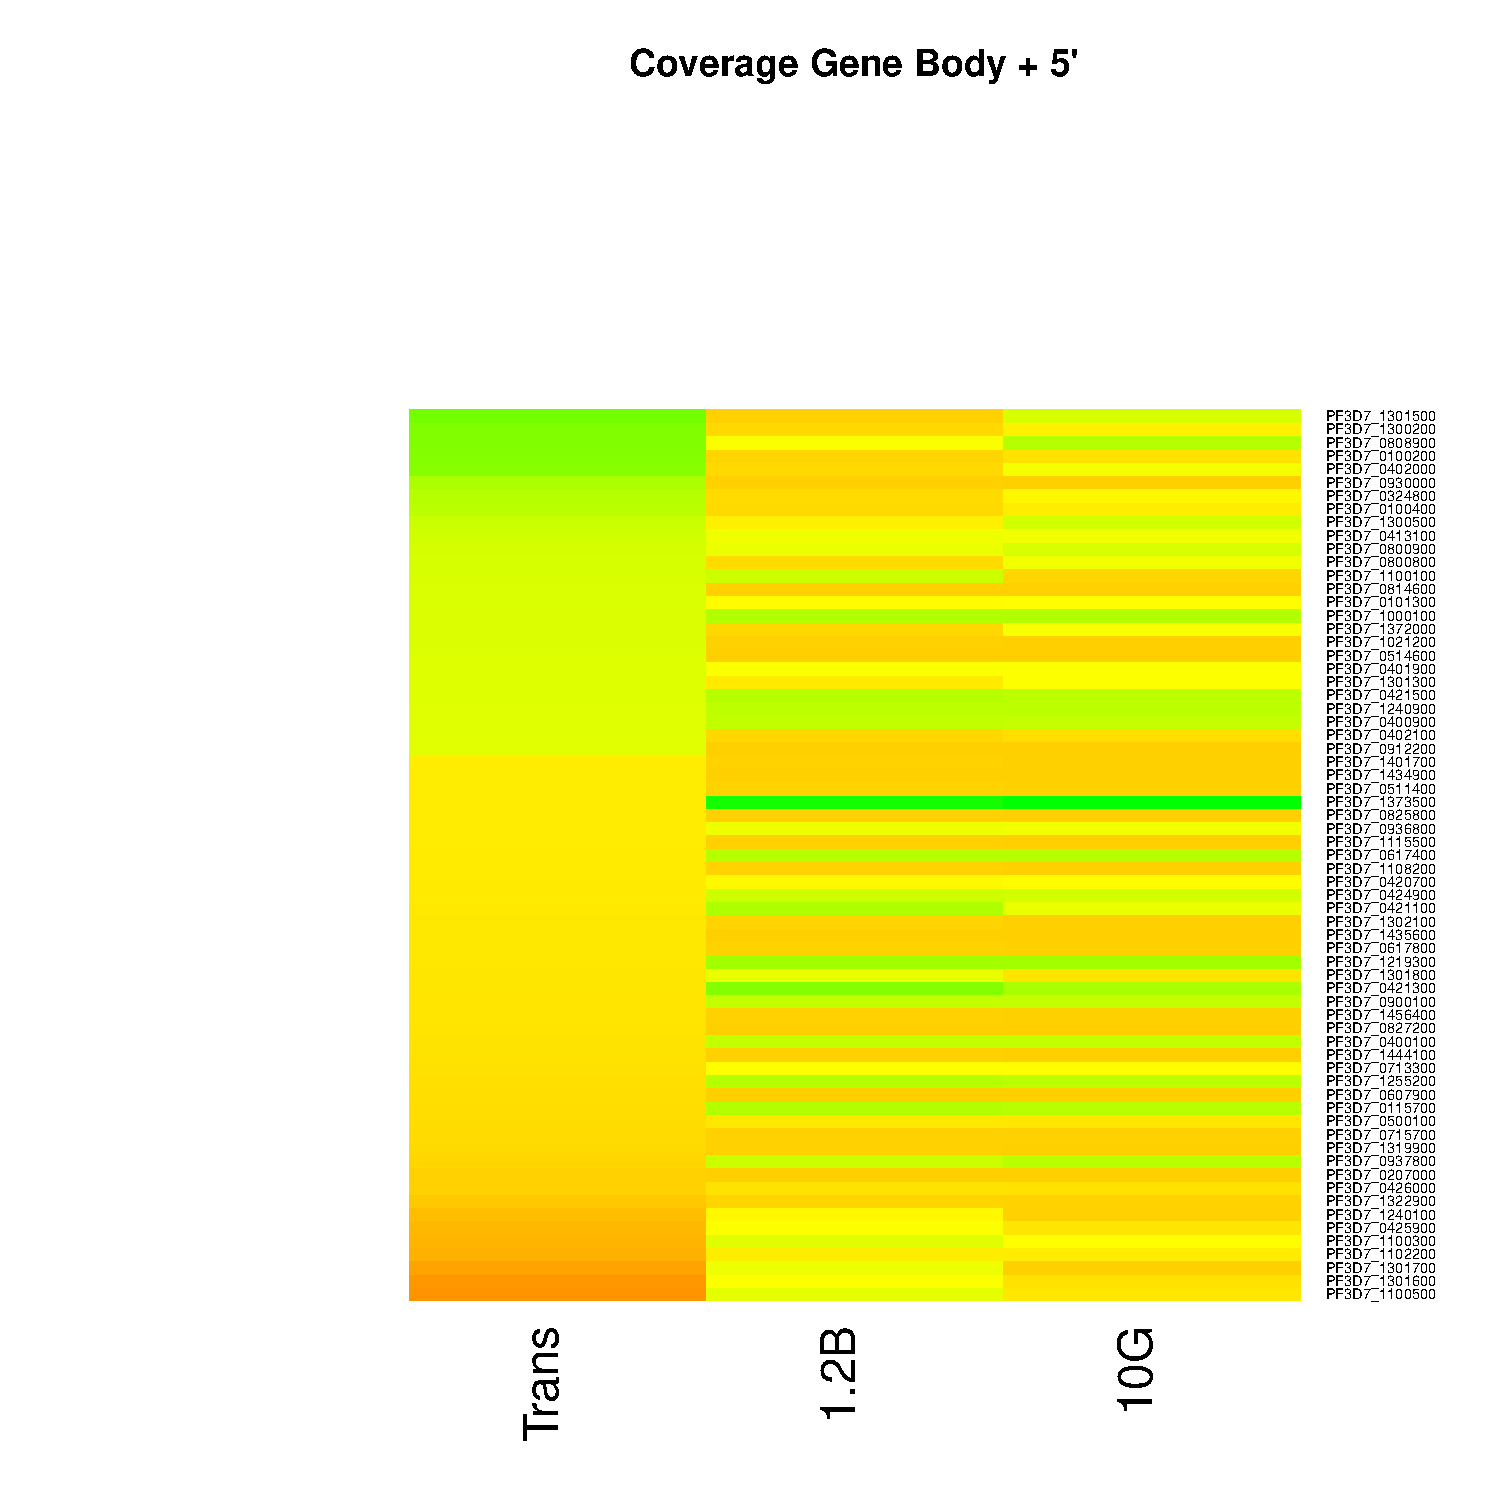
\includegraphics[width=.9\linewidth]{figure/minimal-heat_cov_tss_gene-1} 

}



\end{knitrout}
\clearpage
\subsection{Coverage 3'}
\begin{knitrout}
\definecolor{shadecolor}{rgb}{0.969, 0.969, 0.969}\color{fgcolor}

{\centering 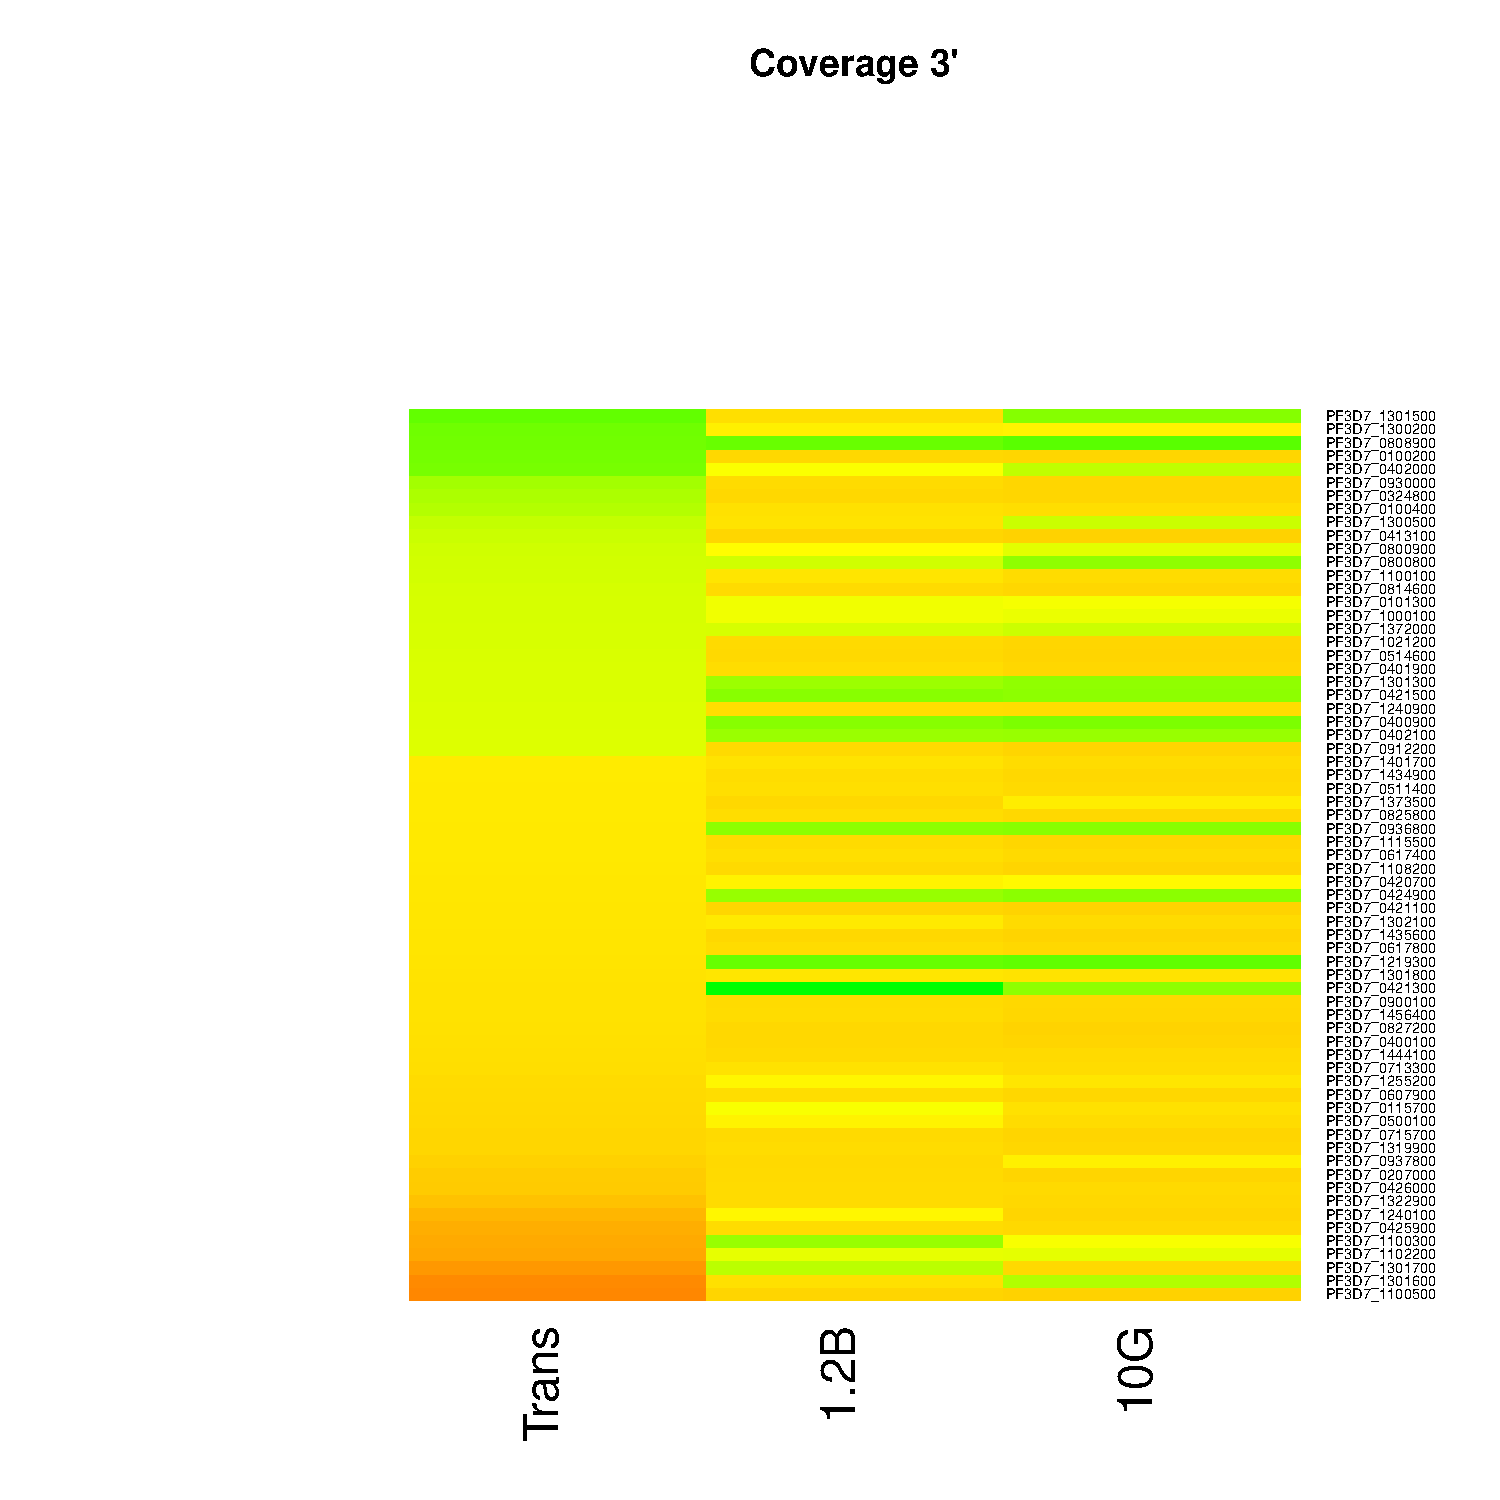
\includegraphics[width=.9\linewidth]{figure/minimal-heat_cov_tts-1} 

}



\end{knitrout}
\clearpage
\subsection{Diferència de Coverage, filtrat per diferència de transcripció}
\begin{knitrout}
\definecolor{shadecolor}{rgb}{0.969, 0.969, 0.969}\color{fgcolor}

{\centering 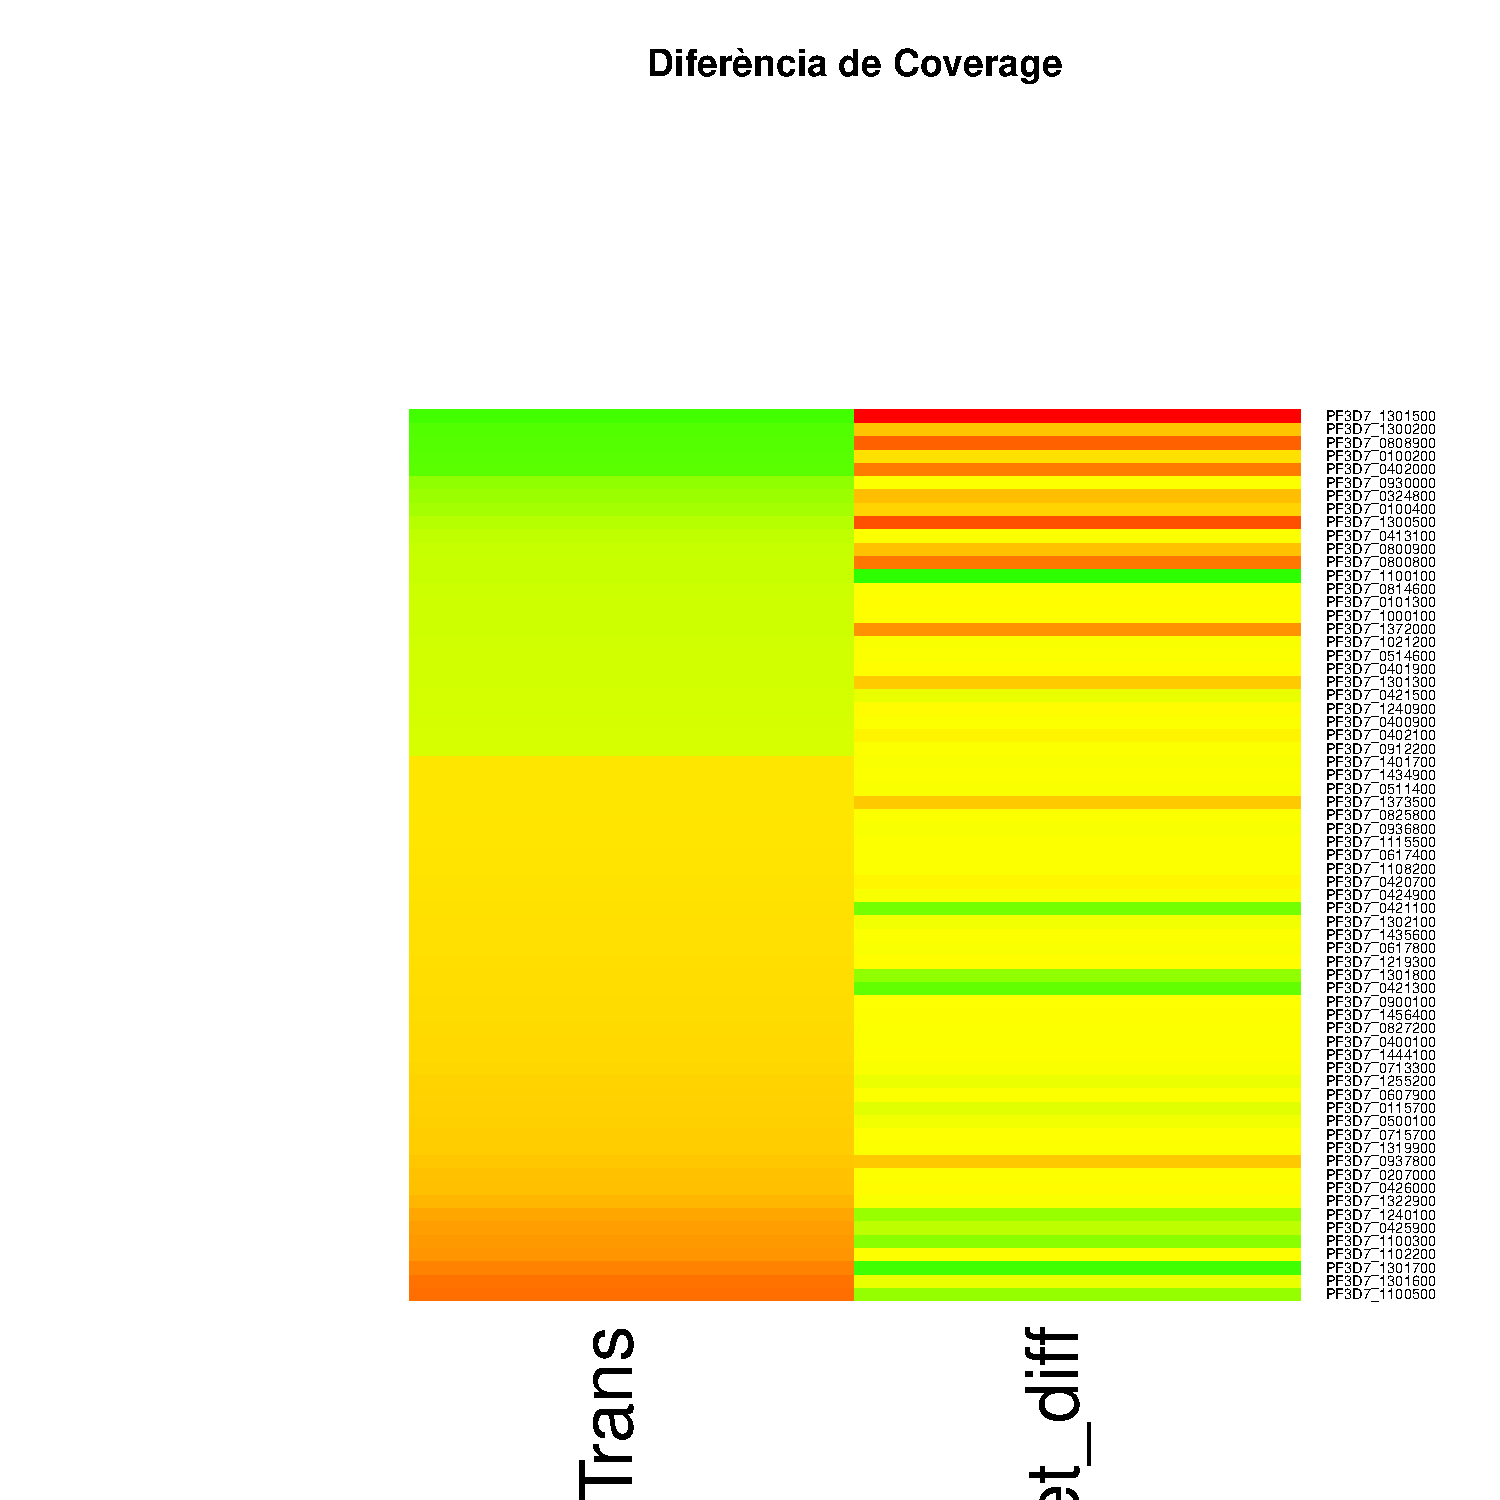
\includegraphics[width=.9\linewidth]{figure/minimal-_heat_cov_diff-1} 

}



\end{knitrout}
\clearpage
\subsection{Diferència de Coverage a 5', filtrat per diferència de transcripció}
\begin{knitrout}
\definecolor{shadecolor}{rgb}{0.969, 0.969, 0.969}\color{fgcolor}

{\centering 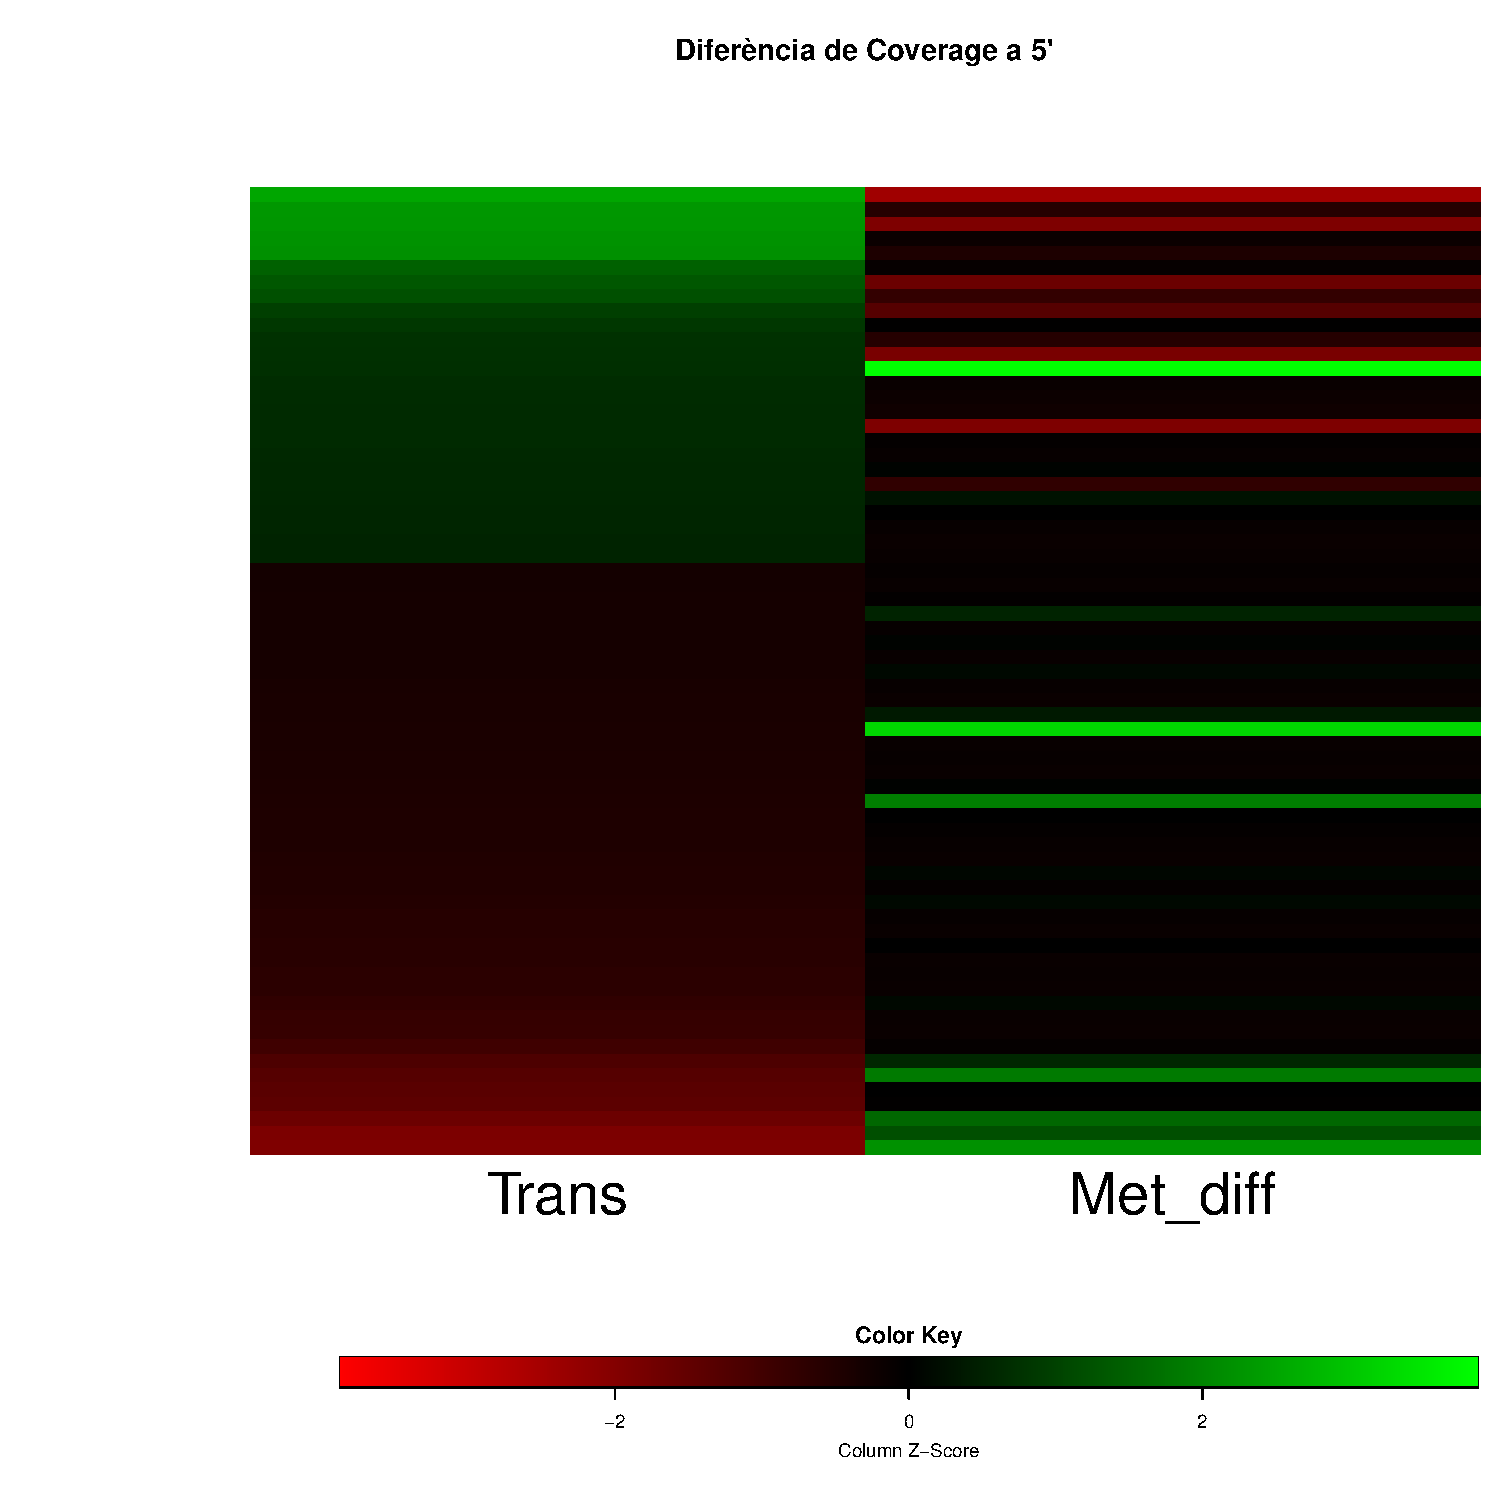
\includegraphics[width=.9\linewidth]{figure/minimal-_heat_cov_diff_5-1} 

}



\end{knitrout}
\clearpage
\subsection{Diferència de Coverage a genebody, filtrat per diferència de transcripció}
\begin{knitrout}
\definecolor{shadecolor}{rgb}{0.969, 0.969, 0.969}\color{fgcolor}

{\centering 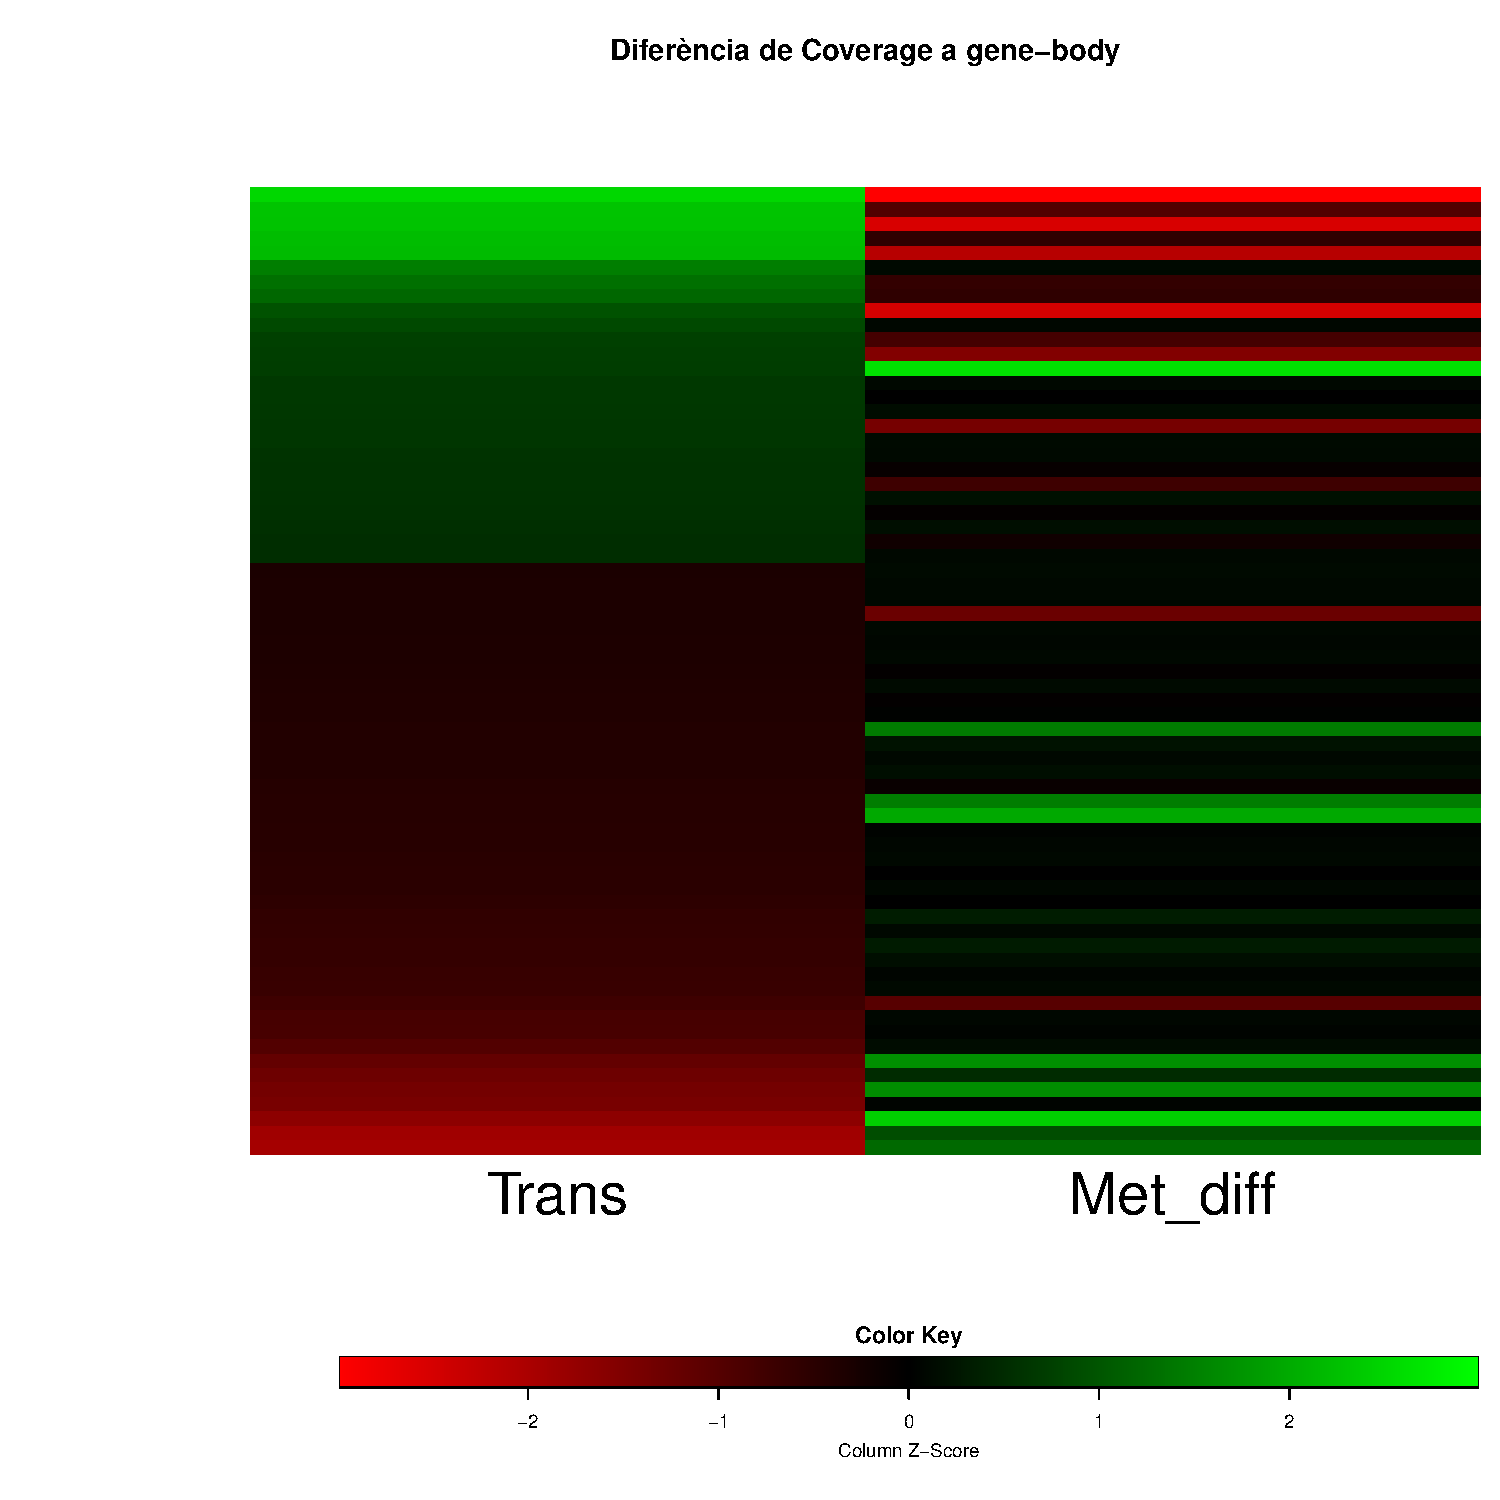
\includegraphics[width=.9\linewidth]{figure/minimal-_heat_cov_diff_body-1} 

}



\end{knitrout}
\clearpage
\subsection{Diferència de Coverage 5'genebody, filtrat per diferència de transcripció}
\begin{knitrout}
\definecolor{shadecolor}{rgb}{0.969, 0.969, 0.969}\color{fgcolor}

{\centering 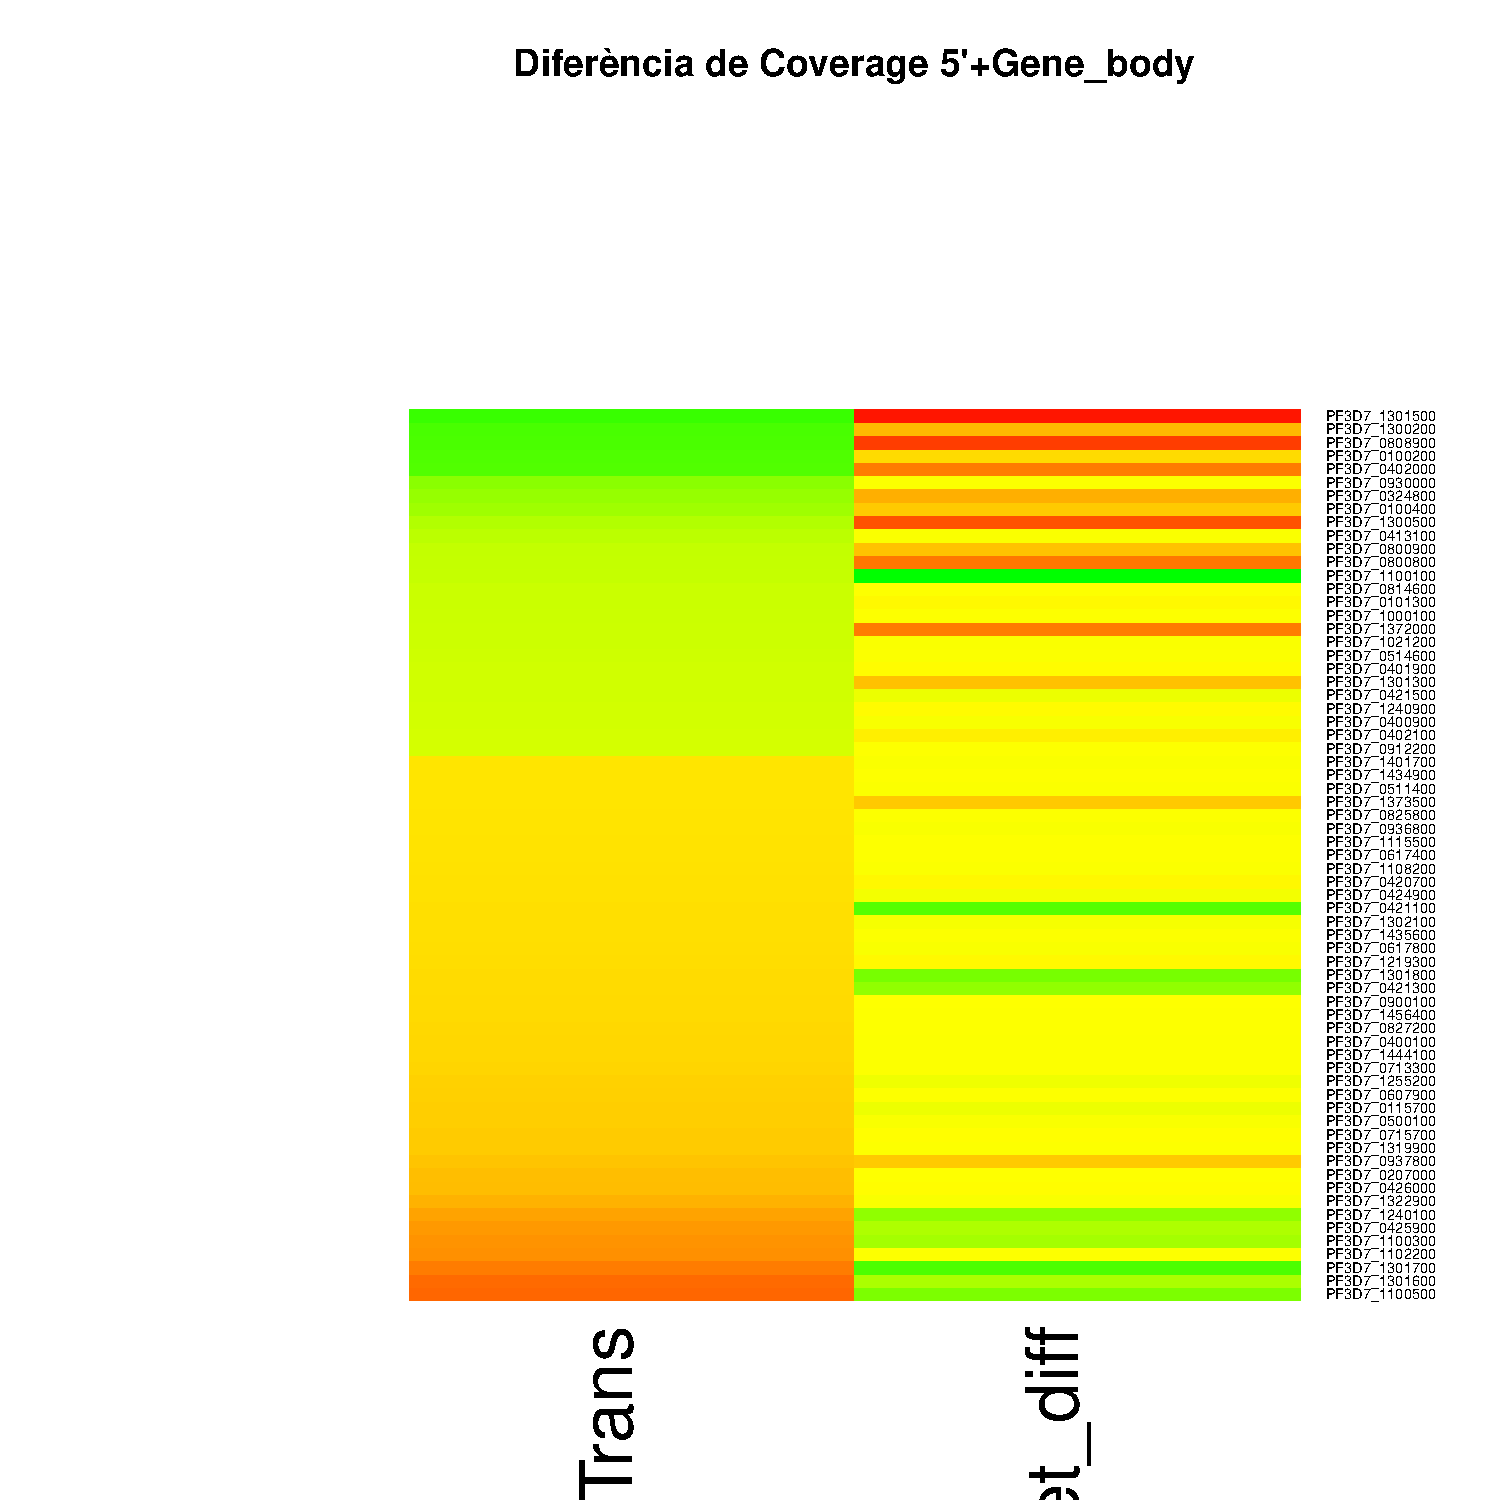
\includegraphics[width=.9\linewidth]{figure/minimal-_heat_cov_diff_body5-1} 

}



\end{knitrout}
\clearpage
\subsection{Diferència de Coverage a 3', filtrat per diferència de transcripció}
\begin{knitrout}
\definecolor{shadecolor}{rgb}{0.969, 0.969, 0.969}\color{fgcolor}

{\centering 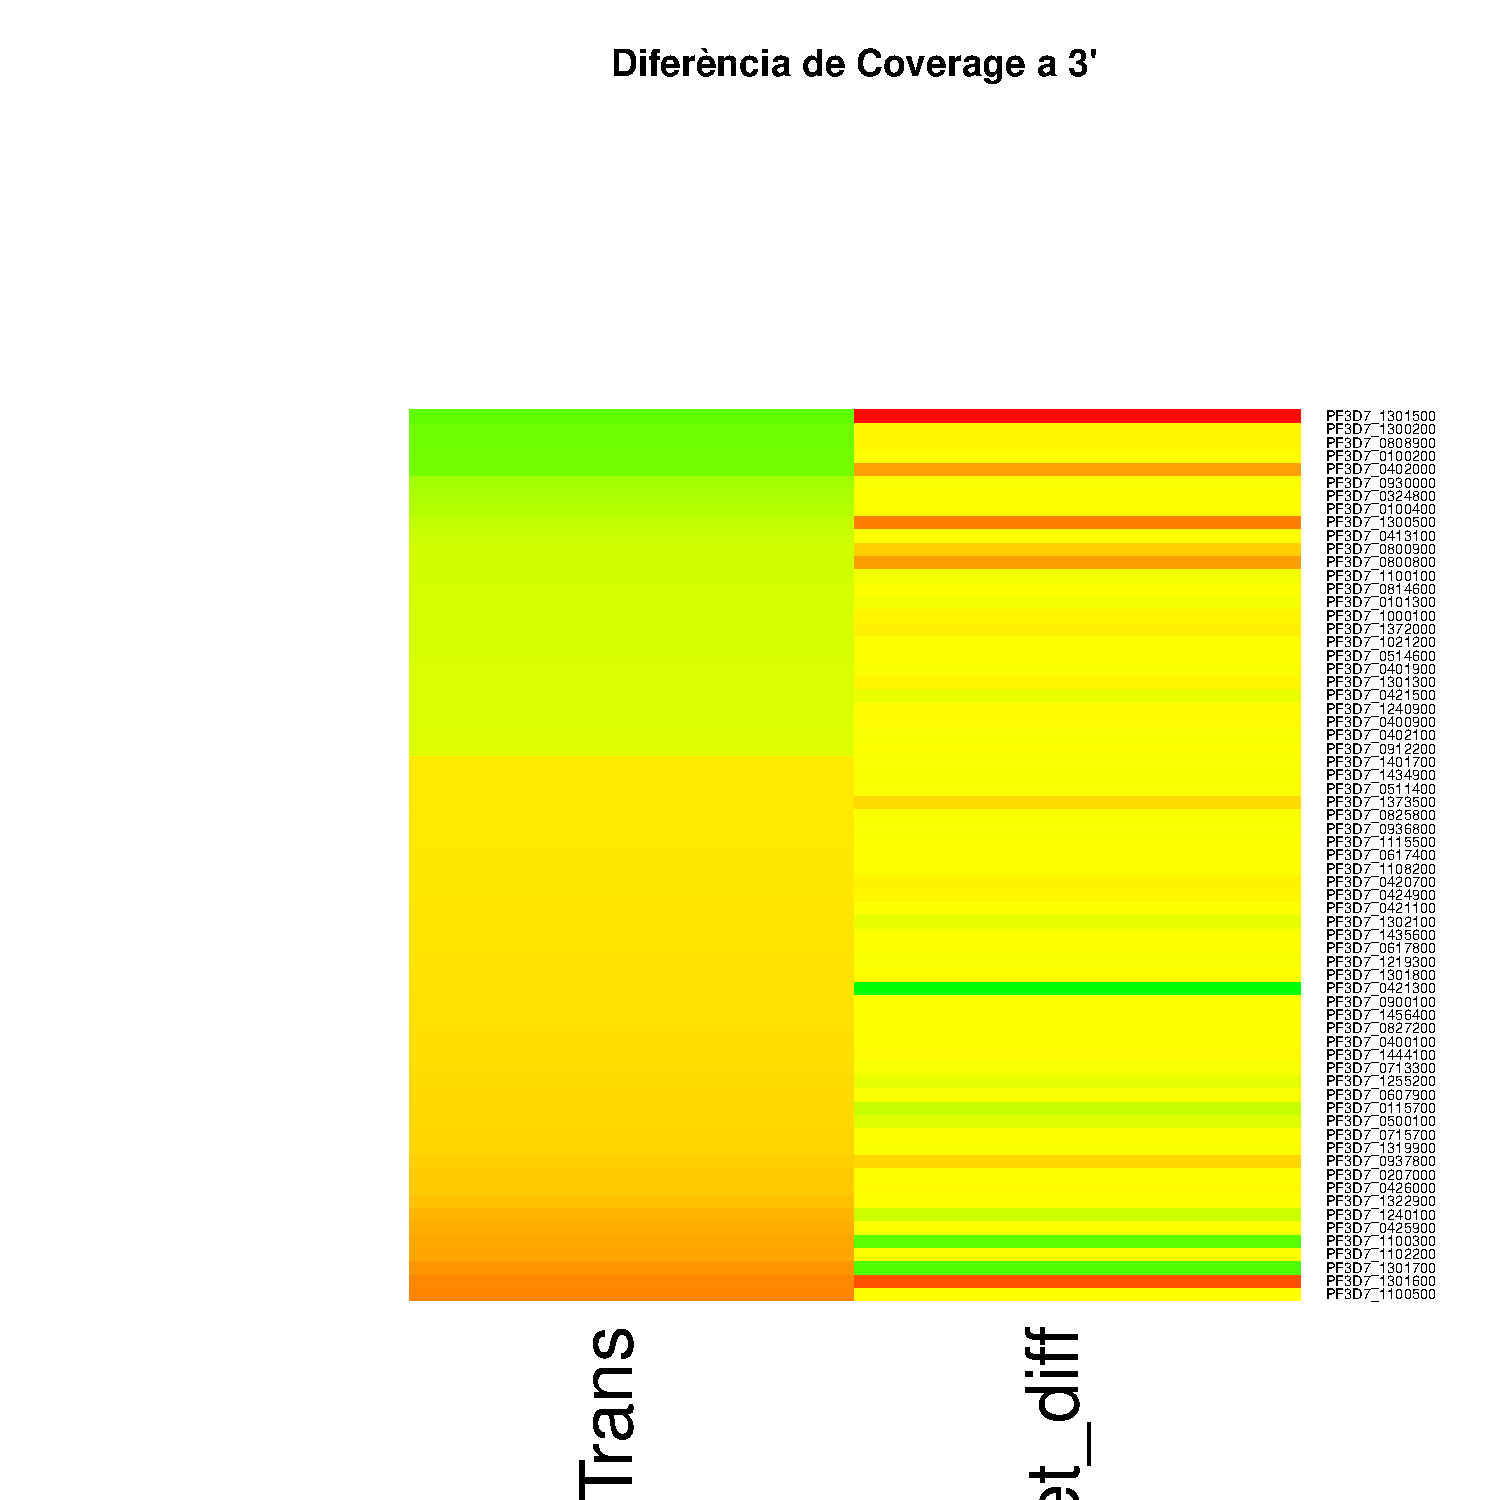
\includegraphics[width=.9\linewidth]{figure/minimal-_heat_cov_diff_3-1} 

}



\end{knitrout}
\clearpage
\subsection{Diferència de Coverage, filtrat per diferència de metilació}
\begin{knitrout}
\definecolor{shadecolor}{rgb}{0.969, 0.969, 0.969}\color{fgcolor}

{\centering 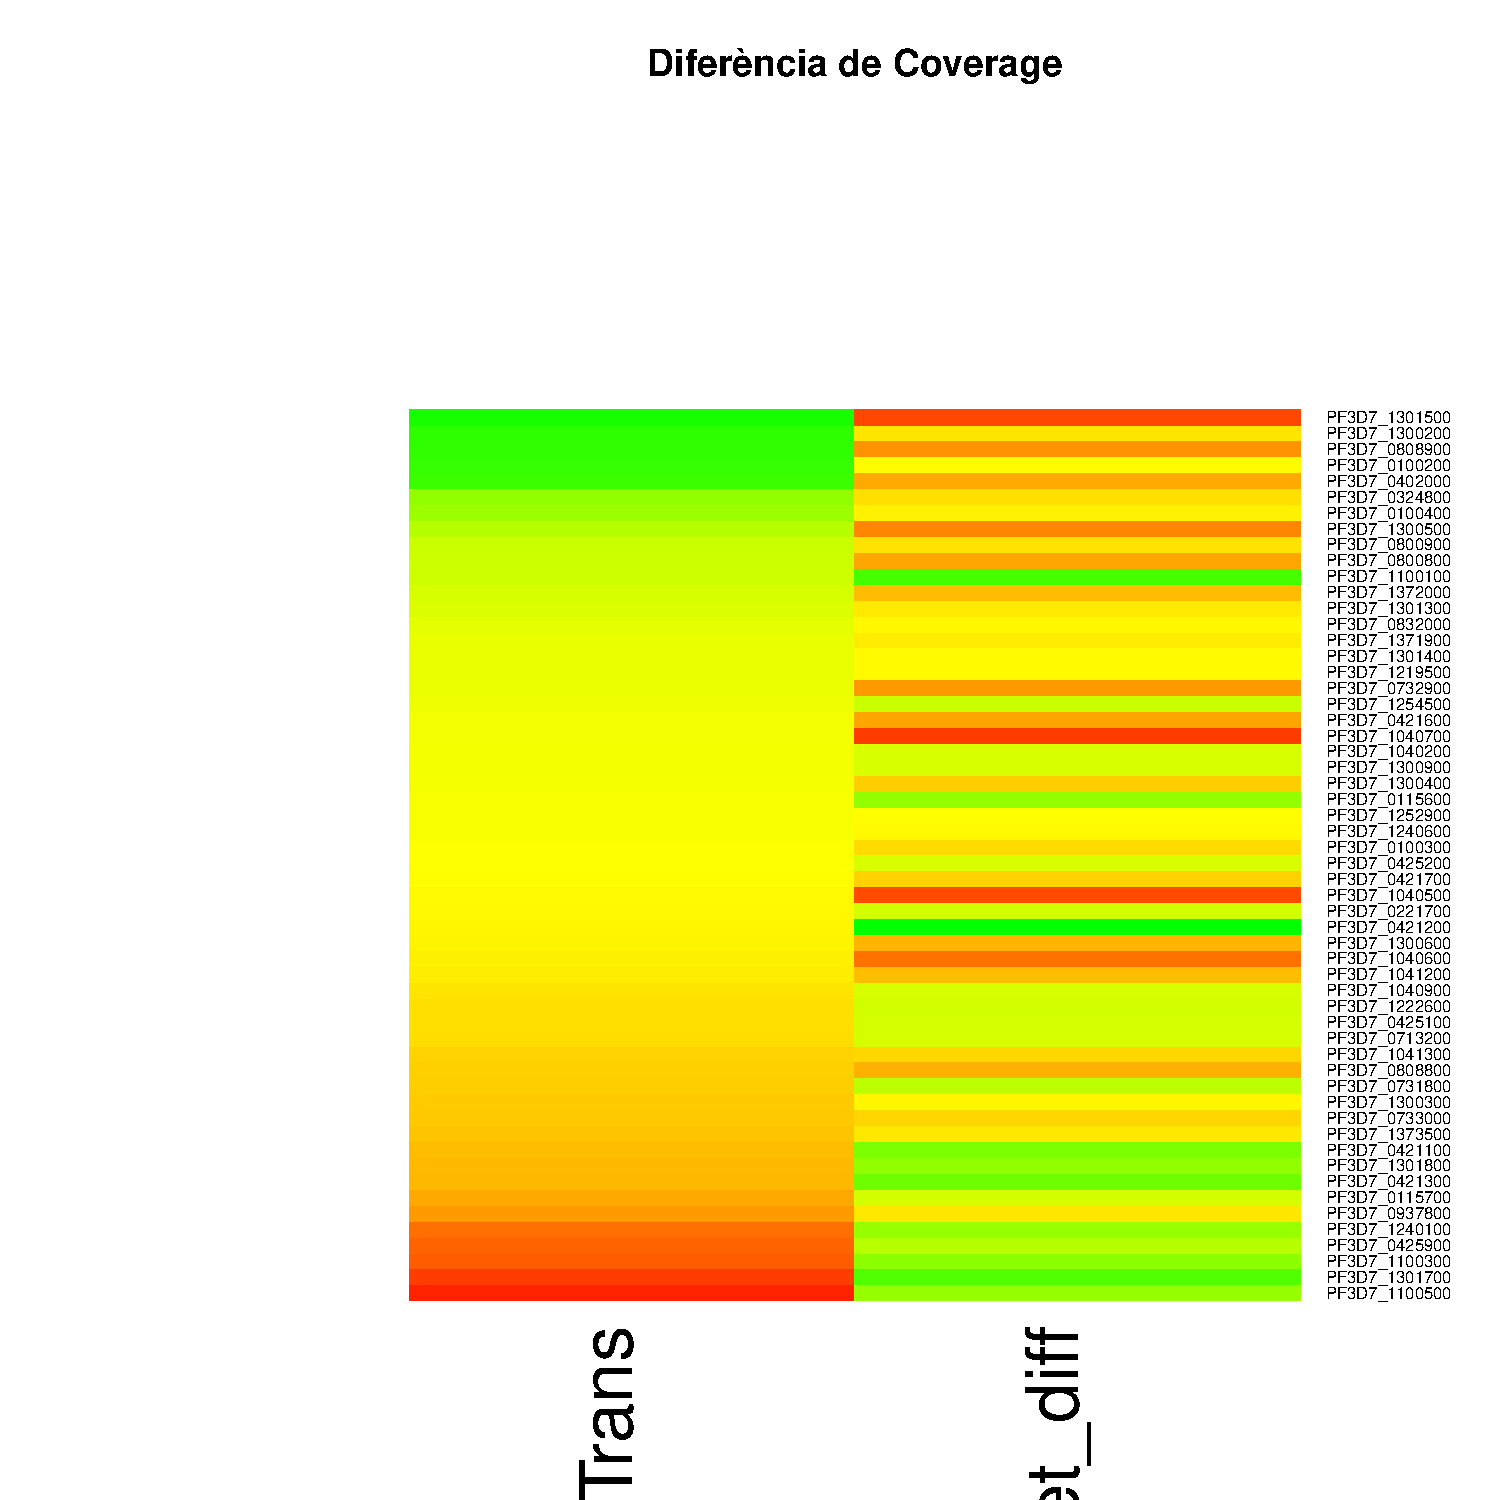
\includegraphics[width=.9\linewidth]{figure/minimal-heat_cov_diff_filter-1} 

}



\end{knitrout}

\clearpage
\section{Coverage a pics diferencials}

\subsection{Heatmaps}
\begin{knitrout}
\definecolor{shadecolor}{rgb}{0.969, 0.969, 0.969}\color{fgcolor}

{\centering 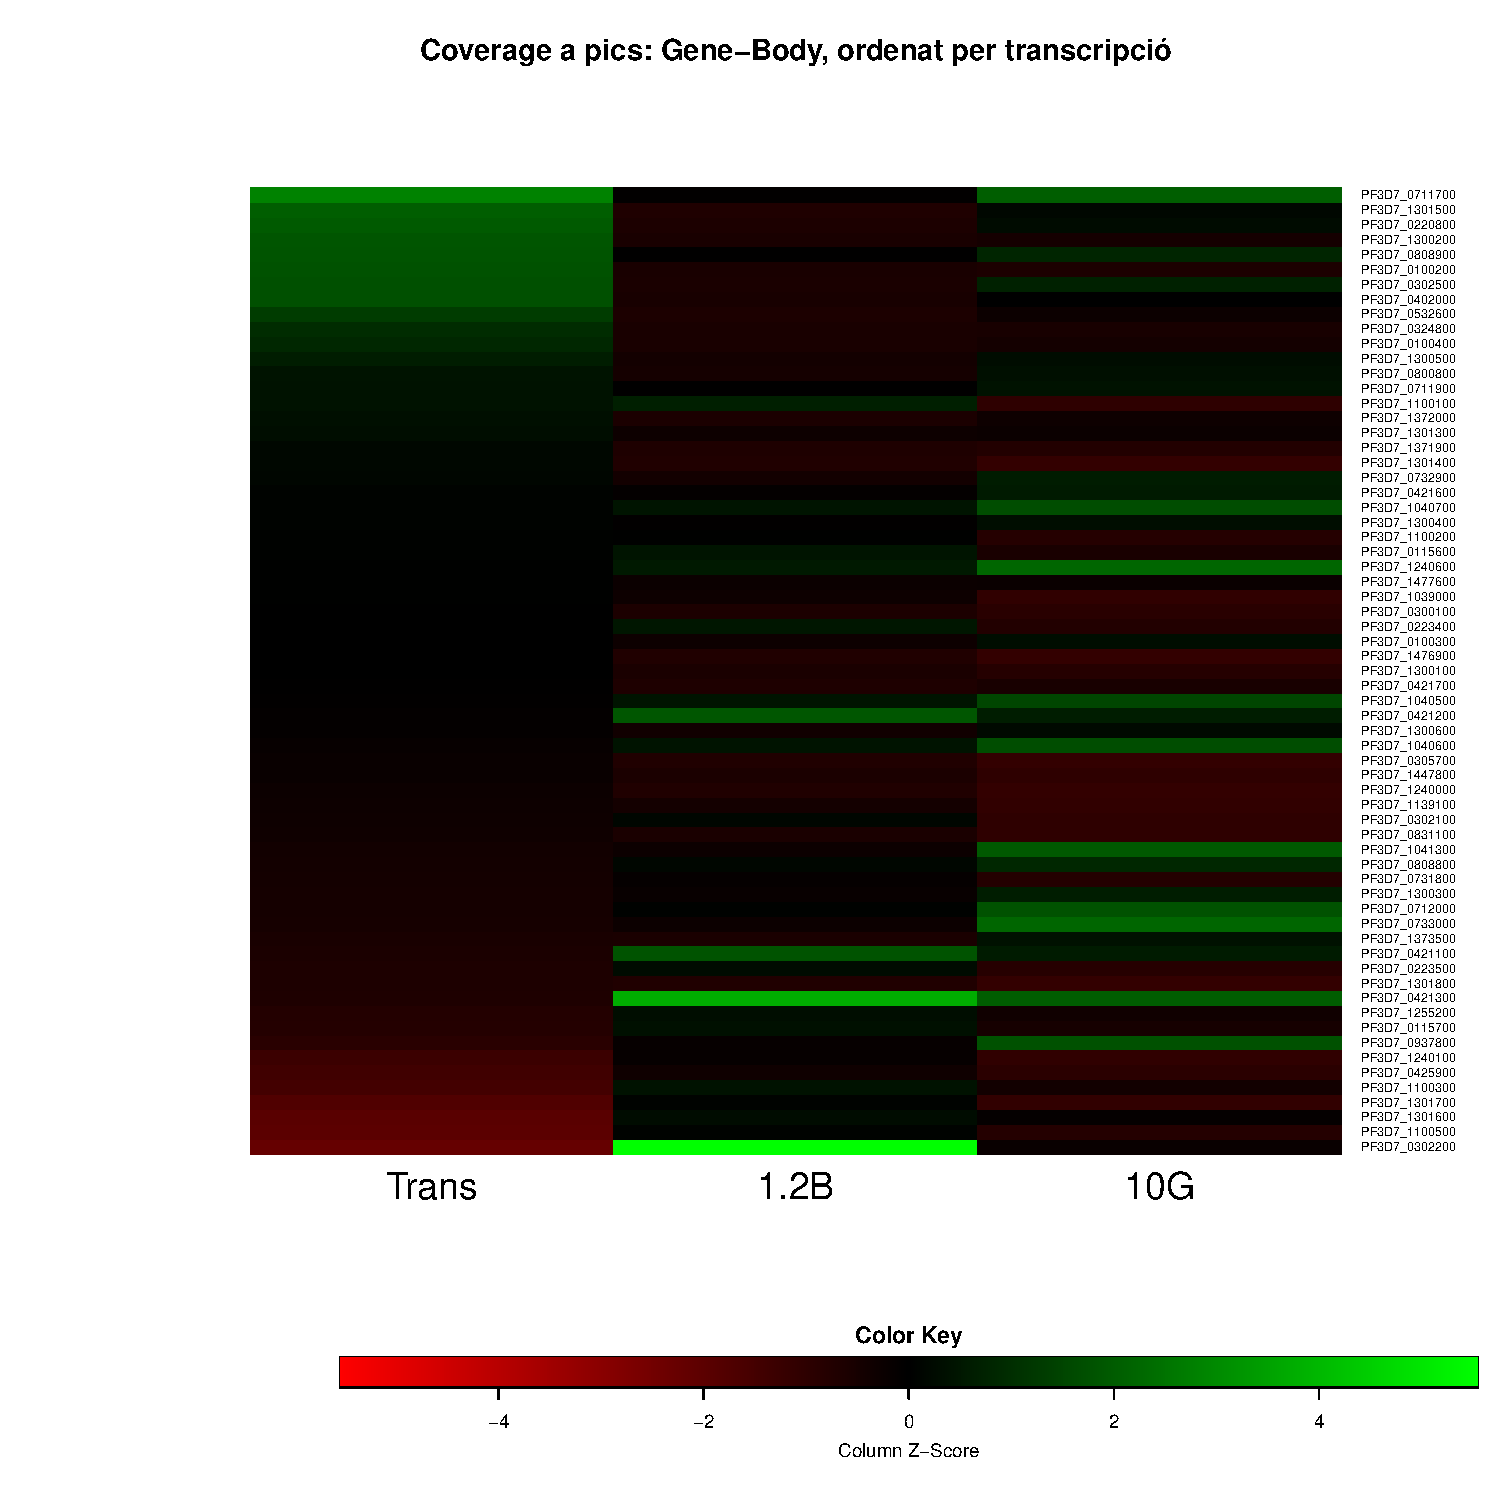
\includegraphics[width=.9\linewidth]{figure/minimal-heat_difpeak_cov-1} 

}



\end{knitrout}
\clearpage
\subsection{Diferència de Metilació}
\begin{knitrout}
\definecolor{shadecolor}{rgb}{0.969, 0.969, 0.969}\color{fgcolor}

{\centering 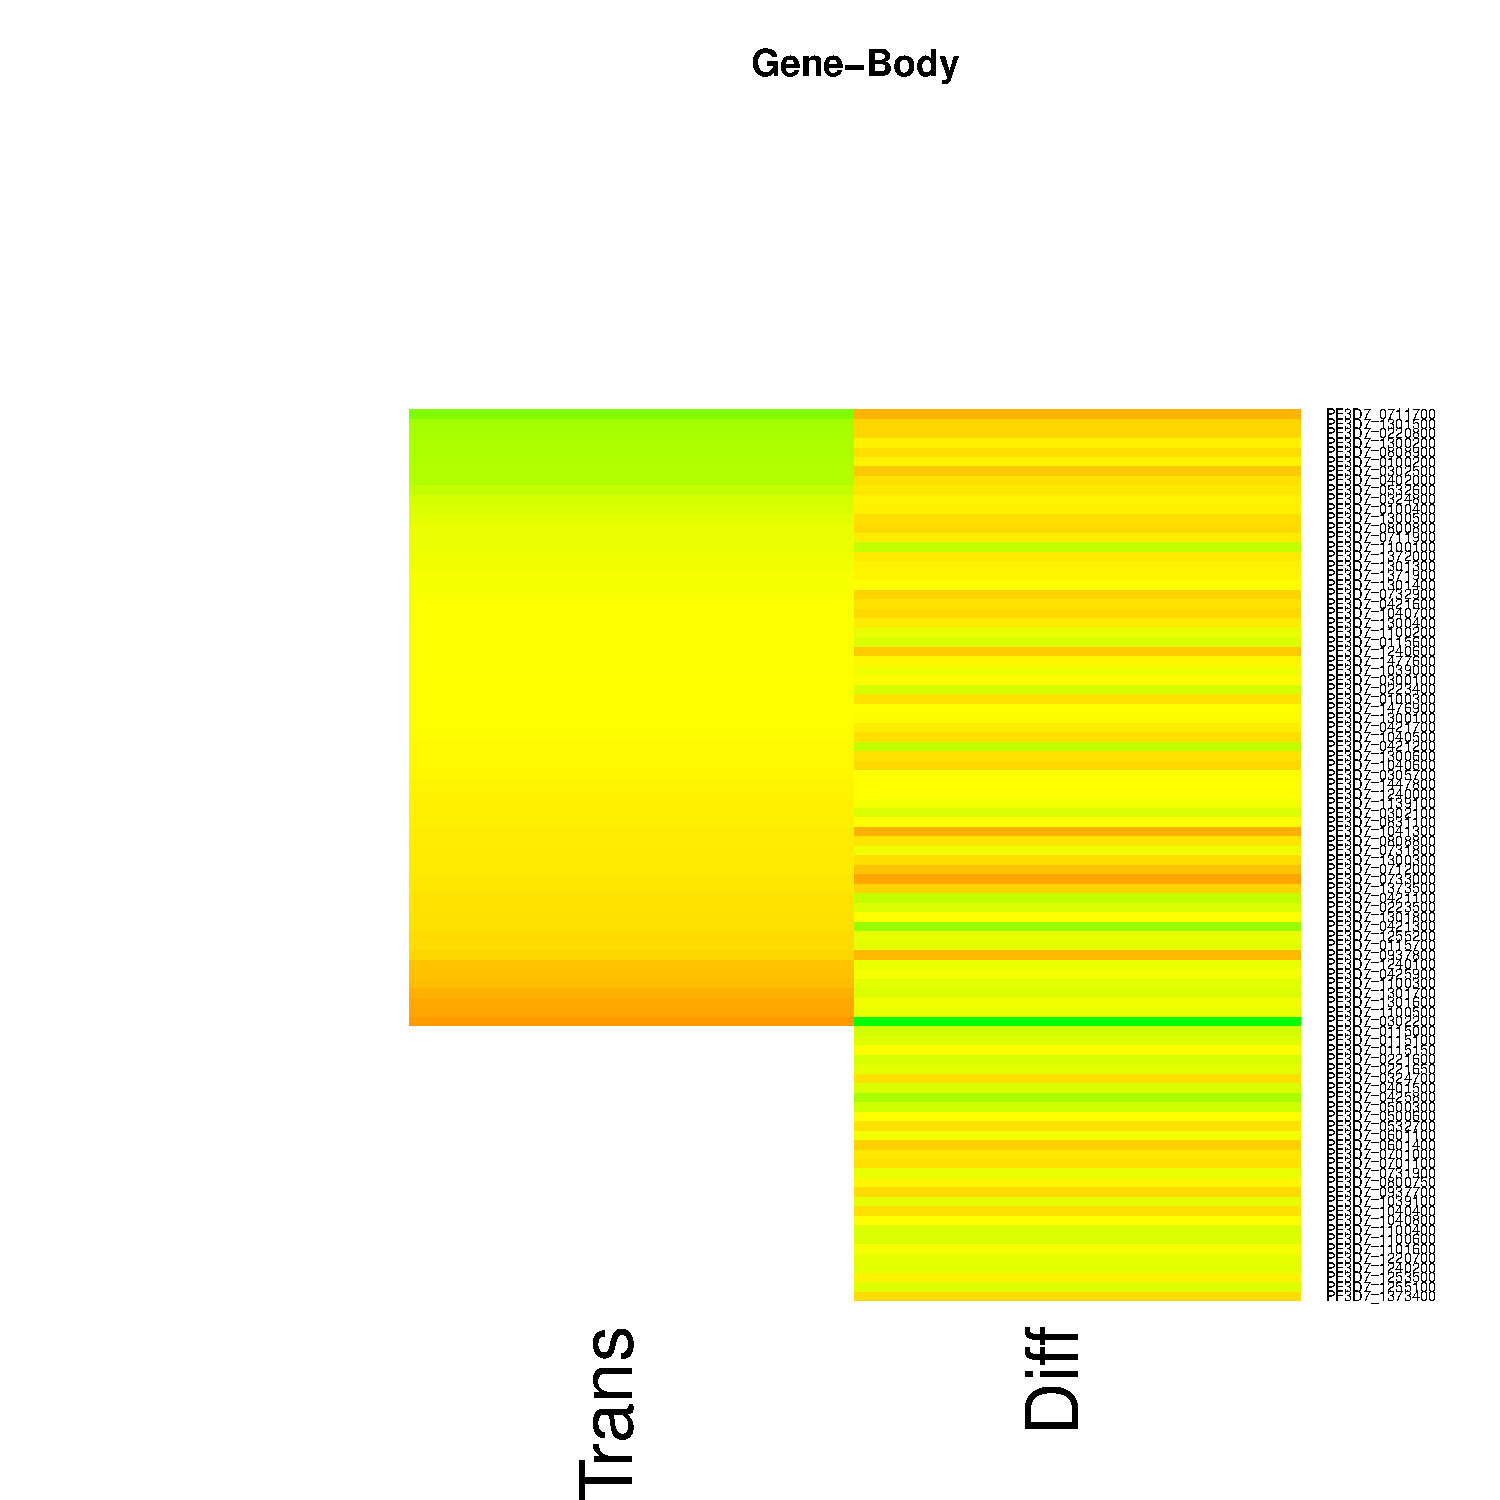
\includegraphics[width=.9\linewidth]{figure/minimal-heat_difpeak_cov_dif-1} 

}



\end{knitrout}
\clearpage
\section{Multiple-regression Model}
\begin{knitrout}
\definecolor{shadecolor}{rgb}{0.969, 0.969, 0.969}\color{fgcolor}\begin{kframe}


{\ttfamily\noindent\bfseries\color{errorcolor}{\#\# Error in `[<-.data.frame`(`*tmp*`, "{}10G\_cov"{}, value = c(219.498997996, : replacement has 94 rows, data has 93}}

{\ttfamily\noindent\bfseries\color{errorcolor}{\#\# Error in `[<-.data.frame`(`*tmp*`, "{}1.2B\_cov"{}, value = c(95.9679358717, : replacement has 94 rows, data has 93}}

{\ttfamily\noindent\bfseries\color{errorcolor}{\#\# Error in model.frame.default(formula = met\_cov\_df\$Trans \textasciitilde{} met\_cov\_df\$`10G` + : invalid type (NULL) for variable 'met\_cov\_df\$`10G\_cov`'}}

{\ttfamily\noindent\bfseries\color{errorcolor}{\#\# Error in model.frame.default(formula = met\_cov\_df\$Trans \textasciitilde{} met\_cov\_df\$`10G` + : invalid type (NULL) for variable 'met\_cov\_df\$`10G\_cov`'}}

{\ttfamily\noindent\bfseries\color{errorcolor}{\#\# Error in model.frame.default(formula = met\_cov\_df\$Trans \textasciitilde{} met\_cov\_df\$`1.2B` + : invalid type (NULL) for variable 'met\_cov\_df\$`1.2B\_cov`'}}

{\ttfamily\noindent\bfseries\color{errorcolor}{\#\# Error in fitted(fit\_all): object 'fit\_all' not found}}

{\ttfamily\noindent\bfseries\color{errorcolor}{\#\# Error in fitted(fit\_10G): object 'fit\_10G' not found}}

{\ttfamily\noindent\bfseries\color{errorcolor}{\#\# Error in fitted(fit\_12B): object 'fit\_12B' not found}}

{\ttfamily\noindent\bfseries\color{errorcolor}{\#\# Error in plot(fit\_all\_df): object 'fit\_all\_df' not found}}

{\ttfamily\noindent\bfseries\color{errorcolor}{\#\# Error in plot(fit\_10G\_df): object 'fit\_10G\_df' not found}}

{\ttfamily\noindent\bfseries\color{errorcolor}{\#\# Error in plot(fit\_12B\_df): object 'fit\_12B\_df' not found}}

{\ttfamily\noindent\bfseries\color{errorcolor}{\#\# Error in rownames(fit\_all\_df) <- met\_cov\_df\$id: object 'fit\_all\_df' not found}}

{\ttfamily\noindent\bfseries\color{errorcolor}{\#\# Error in as.matrix(fit\_all\_df): object 'fit\_all\_df' not found}}\end{kframe}
\end{knitrout}


\end{document}
